% CVPR 2025 Paper Template; see https://github.com/cvpr-org/author-kit

\documentclass[10pt,twocolumn,letterpaper]{article}

%%%%%%%%% PAPER TYPE  - PLEASE UPDATE FOR FINAL VERSION
% \usepackage{cvpr}              % To produce the CAMERA-READY version
\usepackage[review]{cvpr}      % To produce the REVIEW version
% \usepackage[pagenumbers]{cvpr} % To force page numbers, e.g. for an arXiv version

% Import additional packages in the preamble file, before hyperref
\input{preamble}

% It is strongly recommended to use hyperref, especially for the review version.
% hyperref with option pagebackref eases the reviewers' job.
% Please disable hyperref *only* if you encounter grave issues, 
% e.g. with the file validation for the camera-ready version.
%
% If you comment hyperref and then uncomment it, you should delete *.aux before re-running LaTeX.
% (Or just hit 'q' on the first LaTeX run, let it finish, and you should be clear).
\definecolor{cvprblue}{rgb}{0.21,0.49,0.74}
\usepackage[pagebackref,breaklinks,colorlinks,allcolors=cvprblue]{hyperref}

\usepackage{times}  % DO NOT CHANGE THIS
\usepackage{helvet}  % DO NOT CHANGE THIS
\usepackage{courier}  % DO NOT CHANGE THIS
% \usepackage[hyphens]{url}  % DO NOT CHANGE THIS
\usepackage{graphicx} % DO NOT CHANGE THIS
\urlstyle{rm} % DO NOT CHANGE THIS
\def\UrlFont{\rm}  % DO NOT CHANGE THIS
\usepackage{natbib}  % DO NOT CHANGE THIS AND DO NOT ADD ANY OPTIONS TO IT
\usepackage{caption} % DO NOT CHANGE THIS AND DO NOT ADD ANY OPTIONS TO IT
\frenchspacing  % DO NOT CHANGE THIS
\setlength{\pdfpagewidth}{8.5in} % DO NOT CHANGE THIS
\setlength{\pdfpageheight}{11in} % DO NOT CHANGE THIS
\usepackage{xcolor}

\definecolor{pythoncomment}{RGB}{76, 153, 0} % Adjust RGB values as desired
\definecolor{pythonfunction}{RGB}{200, 0, 0} % Red for function names
\definecolor{purpleish}{rgb}{0.5, 0.0, 0.5}

\usepackage{amssymb}
\usepackage{tabularx}
\usepackage{multirow}
\usepackage{booktabs}
\usepackage{subcaption}
\usepackage{algpseudocode}
\usepackage{placeins}

\usepackage{newfloat}
\usepackage{listings}

%
% These are recommended to typeset algorithms but not required. See the subsubsection on algorithms. Remove them if you don't have algorithms in your paper.
\usepackage{algorithm}
% \usepackage{algorithmic}
% \usepackage[ruled,vlined]{algorithm2e}

%
% These are are recommended to typeset listings but not required. See the subsubsection on listing. Remove this block if you don't have listings in your paper.
\usepackage{newfloat}
\usepackage{listings}



%%%%%%%%% PAPER ID  - PLEASE UPDATE
\def\paperID{17112} % *** Enter the Paper ID here
\def\confName{CVPR}
\def\confYear{2025}

%%%%%%%%% TITLE - PLEASE UPDATE
\title{Maximizing Unlabeled Data Utility with Improved Representation Learning and Pseudo Labeling}

%%%%%%%%% AUTHORS - PLEASE UPDATE
\author{First Author\\
Institution1\\
Institution1 address\\
{\tt\small firstauthor@i1.org}
% For a paper whose authors are all at the same institution,
% omit the following lines up until the closing ``}''.
% Additional authors and addresses can be added with ``\and'',
% just like the second author.
% To save space, use either the email address or home page, not both
\and
Second Author\\
Institution2\\
First line of institution2 address\\
{\tt\small secondauthor@i2.org}
}

\begin{document}
\maketitle
\begin{abstract}
An effective semi-supervised approach for representation learning involves two parallel networks - a trainable network and a momentum network. Two augmented versions of the input images go through these networks to predict their outputs and thereby learn the representation. However, this method often fails to maximize its full potential. We identify two major issues regarding data utilization: (1) the need for large batch sizes, which reduces efficiency in memory-constrained environments, and (2) the exclusion of unlabeled data during downstream tasks. We address these limitations with a two-step approach. First, we incorporate both original and augmented images into the trainable network and add a weighted loss term to enhance learning with the additional input. After pre-training, pseudo labels are generated in a meta-learning setup using two identical teacher-student networks, where the teacher network progressively outperforms the student by receiving feedback from it. Our approach, Representation Learning with Pseudo Labeling (RLPL), improves representation learning by achieving higher accuracy for half the batch size of existing methods. RLPL demonstrates an average performance gain of \textbf{6.12\%} across the STL-10, CIFAR-10, and SVHN datasets, with individual improvements ranging from  \textbf{2.7\%} to \textbf{15.74\%}.
\end{abstract}    
\begin{figure*}[!htbp]
  \centering  
  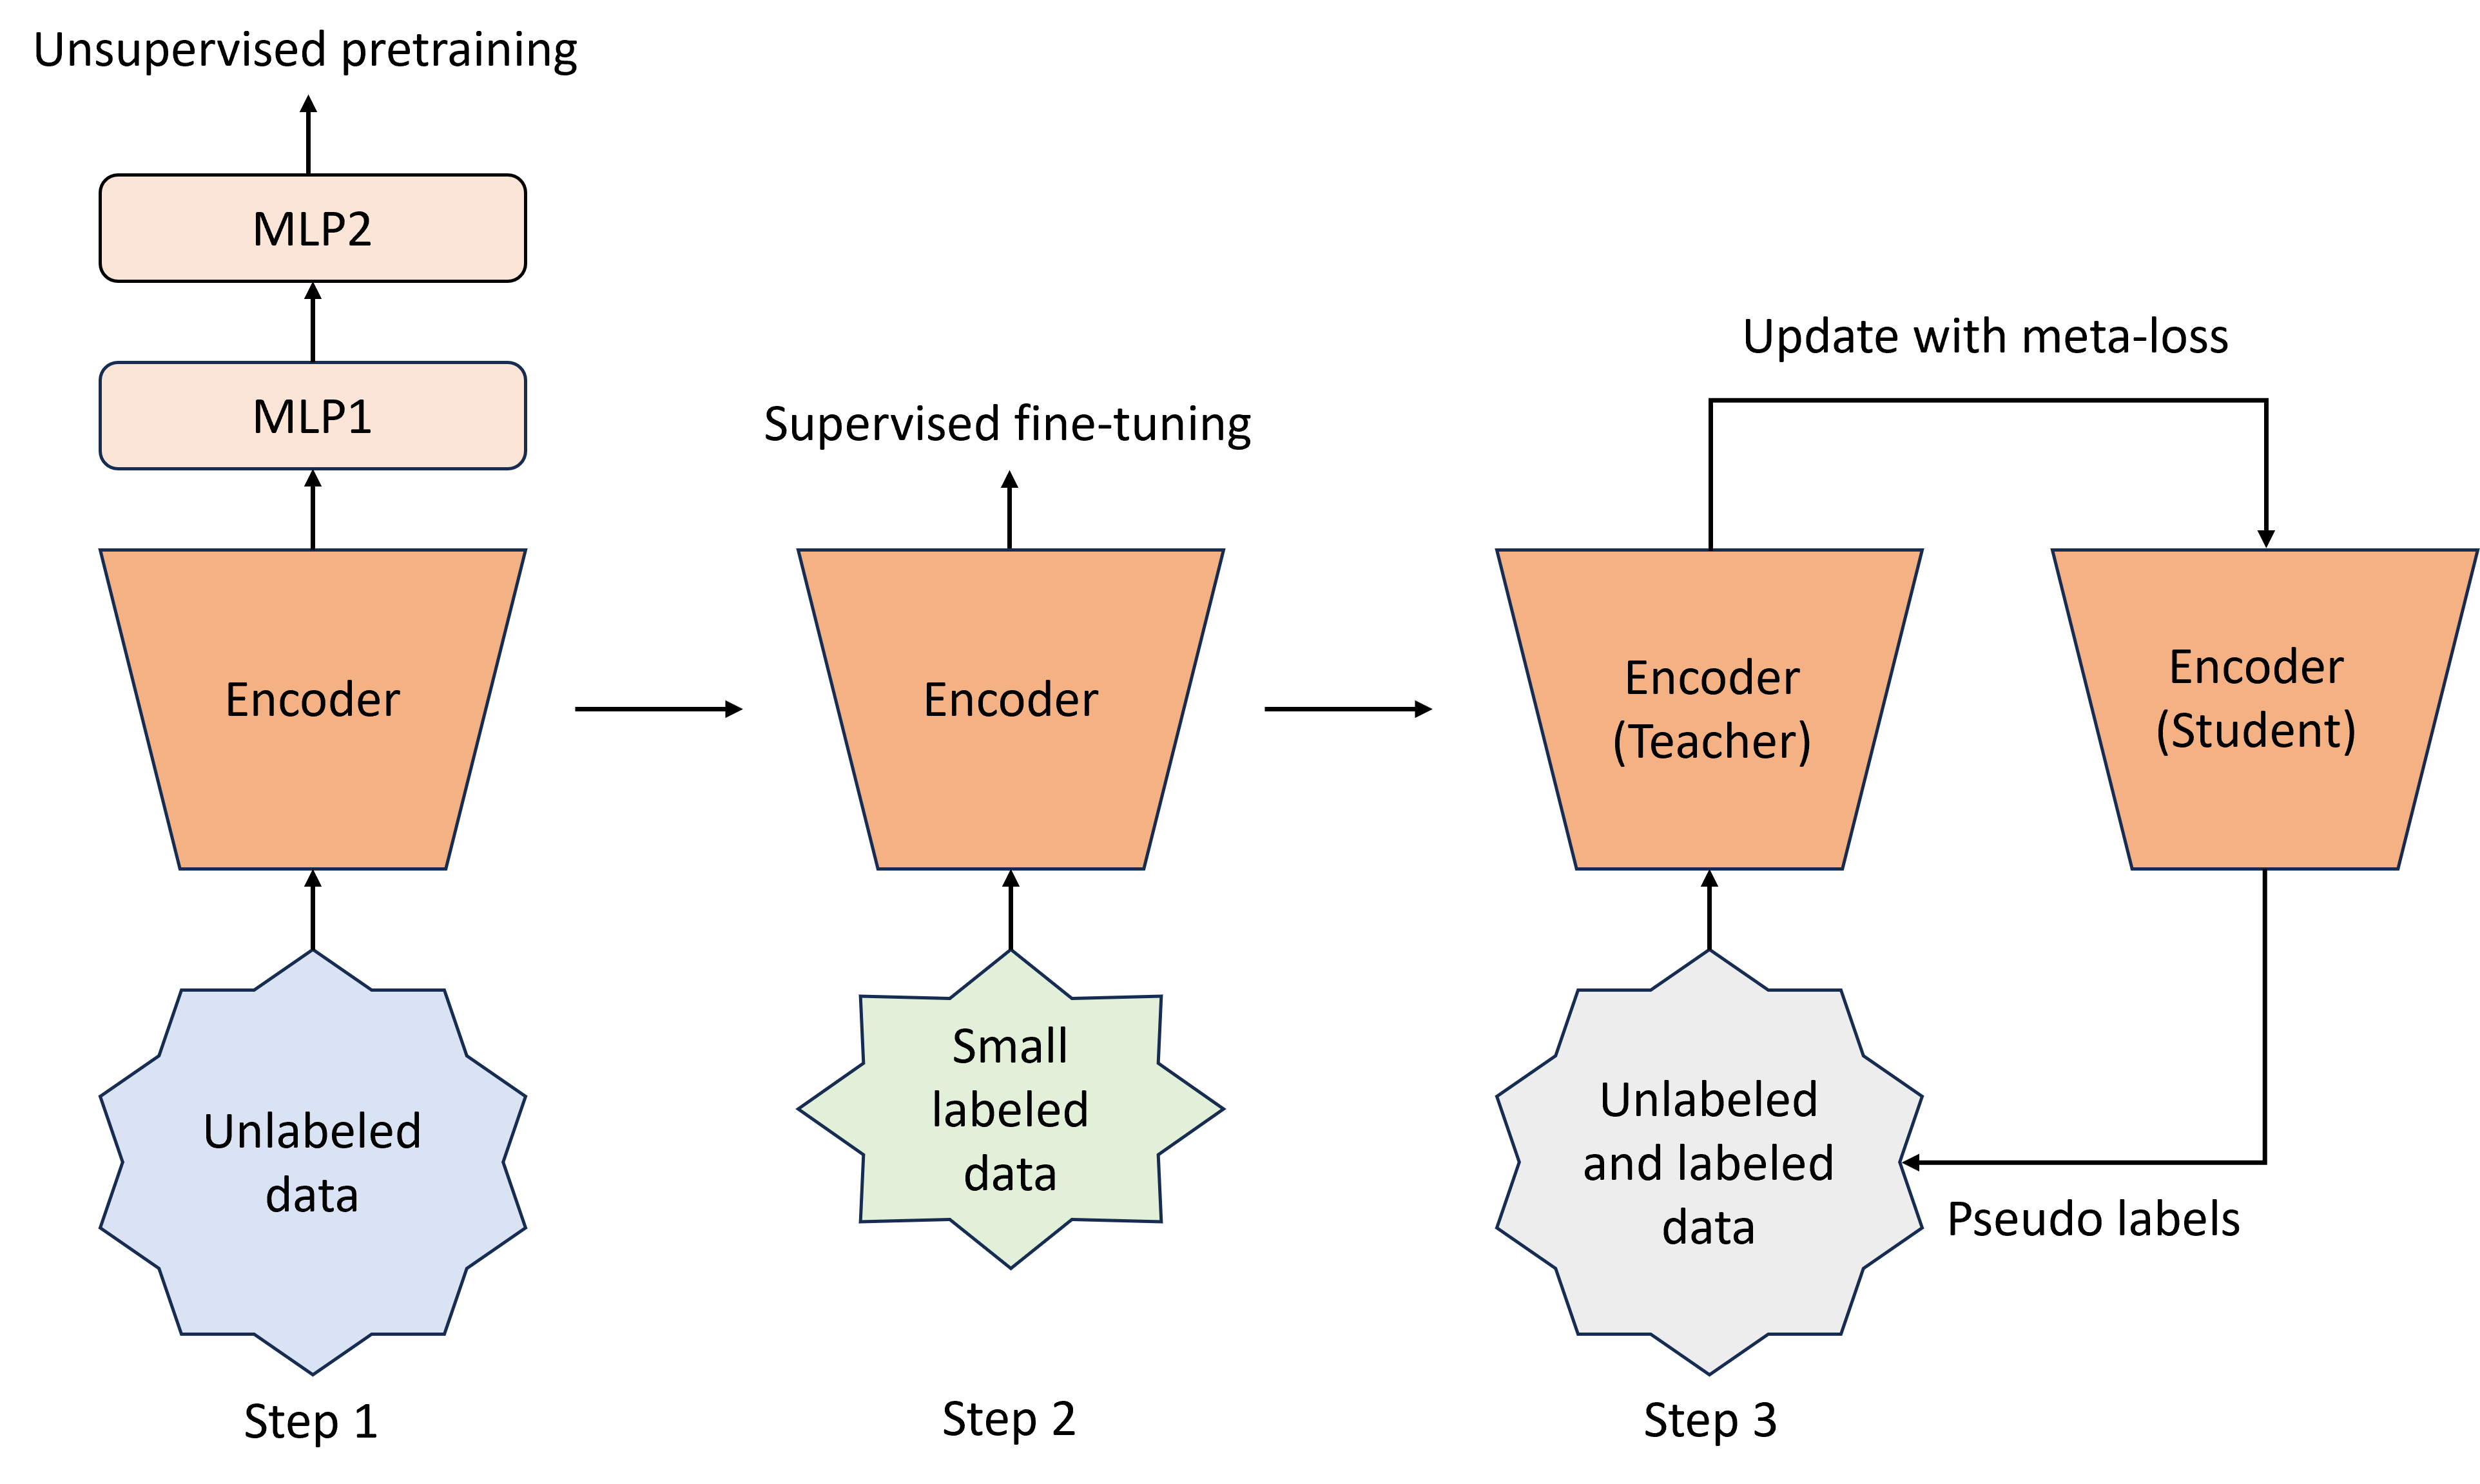
\includegraphics[width=0.75\textwidth]{images/flow.png}
  \caption{\textbf{RLPL flowchart.} 
  RLPL has two levels of unlabeled data utilization. First, it employs unsupervised representation learning. Second, We obtain a highly accurate fine-tuned classifier using only a handful of label data. Lastly, through pseudo labelling using teacher-student networks, both initialized from superior supervised backbone, we improve the classifier further.}
  
% (\textcolor{red}{In this figure, should we indicate the Teacher network with $f_{\theta_T}$, and the Student network with $f_{\theta_S}$? We can mention here at the beginning, $\theta=\theta_T=\theta_S$})
  
  \label{fig:flow}
\end{figure*}
\section{Introduction}

While supervised machine learning algorithms thrive on labeled data, manually annotating this data can be both time-consuming and costly. In contrast, unlabeled data is often readily available and abundant. Although it lacks explicit labels,  unlabeled data still holds valuable information that machine learning models can harness. Semi-supervised learning bridges this gap by extracting meaningful patterns from unlabeled data, compensating for the limited labeled datasets \cite{kingma2014semi}. It achieves this by utilizing the unlabeled data to uncover latent representations—underlying structures and relationships that aren't directly observable. Semi-supervised learning can enhance model performance by incorporating these latent representations, even when labeled data is scarce \cite{devillers2024semi, kutuzova2021multimodal}.

Contrastive learning \cite{chuang2020debiased, fan2023contrastive} has been proven effective in learning the data representation using the unlabeled sample. However, they require negative samples to avoid representational collapse \cite{aghajanyan2020better} and hence were plagued by the problem of mining negative samples \cite{radenovic2023filtering}. There are no apparent methods to obtain effective negative samples, and the presence of higher negative samples than positive ones creates an imbalance \cite{kalantidis2020hard}. Subsequently, contrastive learning methods rely on a large batch size \cite{yang2023batchsampler} to achieve good performance, leading to expensive computational needs.

Representation Learning (RL) methods, such as Bootstrap Your Own Latent (BYOL), SimSiam, and Barlow Twins solve the problem of negative samples by learning representation from the positive class alone. While these methods achieve impressive results with large batch sizes (typically 1024-4096), their performance degrades significantly with smaller batches. This degradation occurs because larger batches provide better gradient estimates and more diverse learning signals, which are crucial for stable representation learning. However, the high memory requirements of large batches make these methods impractical for resource-constrained environments.

Our analysis reveals that the performance drop in existing methods with smaller batches (8-128) stems from two key factors: (1) unstable gradient estimates leading to suboptimal convergence, and (2) limited diversity in the learning signals within each batch. RLPL addresses these challenges through a novel approach that maximizes information utilization from each sample, enabling stable learning even with smaller batches. Through extensive experimentation across different batch sizes, we demonstrate that RLPL maintains consistent performance, showing only a marginal accuracy drop with reduced batch sizes.

Unlabeled data, typically unused in downstream tasks, can enhance performance when leveraged through a model with strong initialization. Pseudo-Labels (PL) \cite{lee2013pseudo} employ a confidence threshold to selectively include those unlabeled samples for which the classifier demonstrates high certainty in its predictions. RL offers an effective initialization, enabling improved model performance and confident pseudo-labeling. However, a notable challenge arises when incorrect pseudo labels are assigned, leading to a degradation in classifier accuracy due to learning from corrupted data. RLPL addresses this issue by refining the pseudo labels through a teacher-student network. This process enhances the teacher network, making it a better model to guide the student network, thereby generating more accurate pseudo labels and boosting overall performance.



% Meta Pseudo Labels (MPL) \cite{Pham_2021_CVPR} addresses pseudo-labeling challenges by iteratively refining PLs through teacher-student \cite{hinton2015distilling} networks, where the teacher network updates itself based on feedback from the student network. Our advanced pseudo-labeling approach focuses on strengthening the teacher network, making it a better model to guide the student network. This improvement helps generate more accurate PLs, which boosts overall performance.

Typical RL methods demand extensive computational resources, such as hundreds of TPUs over several days. Additionally, pseudo-labeling is another memory-heavy method as it uses two networks simultaneously. These requirements are challenging in scenarios where fast, efficient models are needed, like in autonomous vehicles or edge computing \cite{guo2023architecture}. To address these limitations, we implement RLPL on a more manageable batch size and a shallower network, leveraging just two Nvidia 4090 GPUs. Our study shows that RLPL, even without the usage of pseudo labeling, achieves higher accuracy with a batch size of 64, outperforming BYOL with a 128 batch size. Remarkably, RLPL consistently outperforms other RLs with a ResNet18 classifier. RLPL yields average accuracy improvements of \textbf{2.7\%}, \textbf{9.22\%}, and \textbf{4.16\%} that the closest contemporary method on the STL-10, CIFAR-10, and SVHN datasets, respectively.

% Our study shows that RLPL achieves competitive accuracy even with a batch size of 64, matching or outperforming other methods using much larger batches. While methods like FixMatch and MixMatch report higher accuracies (94.83% and 94.41% respectively on STL-10) with large batches (4096), they show significant degradation with smaller batches. In contrast, RLPL maintains robust performance across batch sizes, making it particularly suitable for resource-constrained scenarios. With ResNet18 as the backbone, RLPL yields average accuracy improvements of \textbf{2.7\%}, \textbf{9.22\%}, and \textbf{4.16\%} over the closest contemporary method on the STL-10, CIFAR-10, and SVHN datasets, respectively, when using comparable batch sizes.

Figure \ref{fig:flow} illustrates our framework. In summary, our work contains the following contributions:

\begin{itemize}

\item Our approach cleverly leverages most information from the inputs, leading to enhanced global representation learning. By making this strategic adjustment, our model achieves improved representations with a smaller batch size, ultimately achieving higher accuracy in the downstream tasks.

\item During the downstream task, we utilize unlabeled samples a second time with pseudo labeling. Our approach uses the student network feedback with a meta-loss update to improve the noisy teacher \cite{xie2020self} as the final classifier.

\item RLPL outperforms other State-Of-The-Art (SOTA) RL algorithms on an equivalent but more compact architecture, making it more efficient and cost-effective for edge computing in resource-constrained environments.

\end{itemize}
\section{Related Work}

\subsection{Representation Learning}

Representation learning is a powerful technique for uncovering hidden features in unlabeled data, gaining popularity over time \cite{scholkopf2021toward,hamilton2017representation,le2020contrastive}. Initial methods, like auto-encoders \cite{zhang2019aet, goyal2017nonparametric} and adversarial learning \cite{sarafianos2019adversarial,radford2015unsupervised,donahue2019large} from image samples, have their challenges. They often demand detailed inputs and hefty computational resources. Moreover, their outputs end up in pixel space instead of the more practical feature space, limiting their usefulness for downstream tasks.

A more contemporary approach to representation learning, contrastive learning \cite{tian2020makes,chuang2020debiased}, has demonstrated greater effectiveness. Contrastive learning operates by bringing similar images together while pushing dissimilar ones apart. Supervised contrastive learning \cite{khosla2020supervised} executes in a fully supervised setting, leveraging label information to improve clustering in embedding space and achieve superior performance. The proposed Supervised Contrastive (SupCon) loss outperforms traditional cross-entropy loss on various datasets and demonstrates robustness to natural corruptions and stability to hyperparameter changes. On the other hand, Unsupervised Data Augmentation (UDA) \cite{xie2020unsupervised}  utilizes semi-supervised learning by enhancing the quality of noise through advanced data augmentation methods, significantly boosting model performance on various tasks. An influential algorithm in this domain, SimCLR \cite{chen2020simple}, employs positive and negative image pairs for contrastive learning in a semi-supervised manner. SimCLR has exhibited remarkable performance, achieving SOTA accuracy on the ImageNet \cite{deng2009imagenet} dataset. However, SimCLR comes with significant computational expenses due to its reliance on large batch sizes and the incorporation of positive and negative pairs. These limitations render SimCLR impractical for many applications.

BYOL, SimSiam, Barlow Twin, and Momentum Contrast (MoCo) \cite{he2019momentum} are put forward as more efficient alternatives to SimCLR. A notable departure from SimCLR is eliminating the need for negative pairs during training. Instead, they leverage a pair of augmented views of the same image, streamlining the training process and reducing computational overhead. This design choice positions these RL algorithms as computationally more efficient options than SimCLR. SimCLRv2 \cite{chen2020big} uses a big pretrained model for a second stage data utilization.  In contrast, our approach eliminates the reliance on large models by maintaining a consistent model architecture across all training phases.

\subsection{Pseudo Labeling}

In semi-supervised learning, pseudo-labeling is used on a highly accurate classifier to label and learn from it. This approach has proven effective in various applications like object detection \cite{li2022rethinking,yan2019semi}, image classification \cite{taherkhani2021self,wu2017semi}, and speech recognition \cite{lugosch2022pseudo}. If pseudo labels are inaccurately assigned, classifiers may learn from erroneous labels, diminishing their performance \cite{arazo2020pseudo}.

Many pseudo-labeling methods focus on enhancing the network through consistency loss \cite{zhang2021flexmatch}, moving away from the traditional approach of retraining the model with pseudo labels \cite{iscen2019label}. Consistency-based methods ensure stable model predictions across various augmented views of the same input \cite{rizve2021defense}. However, consistency loss typically updates the network with a fraction of the cross-entropy loss \cite{wang2023kd}, reducing its impact. This diminished emphasis on consistency loss can hinder the network's optimal update, as it does not fully leverage retraining with pseudo labels \cite{xie2020unsupervised}.

MPL addresses the issue of incorrect pseudo-labeling by applying a meta-learning \cite{lee2019meta} approach. In MPL, the teacher uses its softmax predictions on unlabeled data to instruct the student. These predictions, commonly called soft labels, are a well-established concept in the literature on knowledge distillation \cite{cho2019efficacy,phuong2019towards}. This additional adaptation empowers the teacher to generate more accurate PLs for instructing the student network. MPL employs the same bi-level optimization technique from meta-learning \cite{snell2017prototypical, nichol2018reptile, finn2017model} to iteratively update the teacher-student framework. 

Notably, MPL progressively enhances the student network, while our training focuses more on improving the teacher network. This is because the teacher network receives more frequent feedback and updates - first through feedback from the student and then from the meta loss update. Additionally, introducing a controlled noise in either the teacher or student network is crucial, especially when the two networks are similar. This noise injection boosts the learning process's robustness and generalization \cite{wang2023consistent, li2024nicest}.
\section{Proposed Methodology: RLPL}

\subsection{Improved Representation Learning}

In RLPL, the trainable and momentum networks use identical encoders for image embeddings. These embeddings are projected to a lower-dimensional space using a Multi-Layer Perceptron (MLP) in each network. The momentum network stops here, producing outputs with a dimension of 256. In contrast, the trainable network includes an additional prediction head, consisting of another MLP layer with the same dimension.

\begin{figure*}[!htbp]
    \centering
    % First subfigure
    \begin{subfigure}[b]{0.48\textwidth}
        \centering
        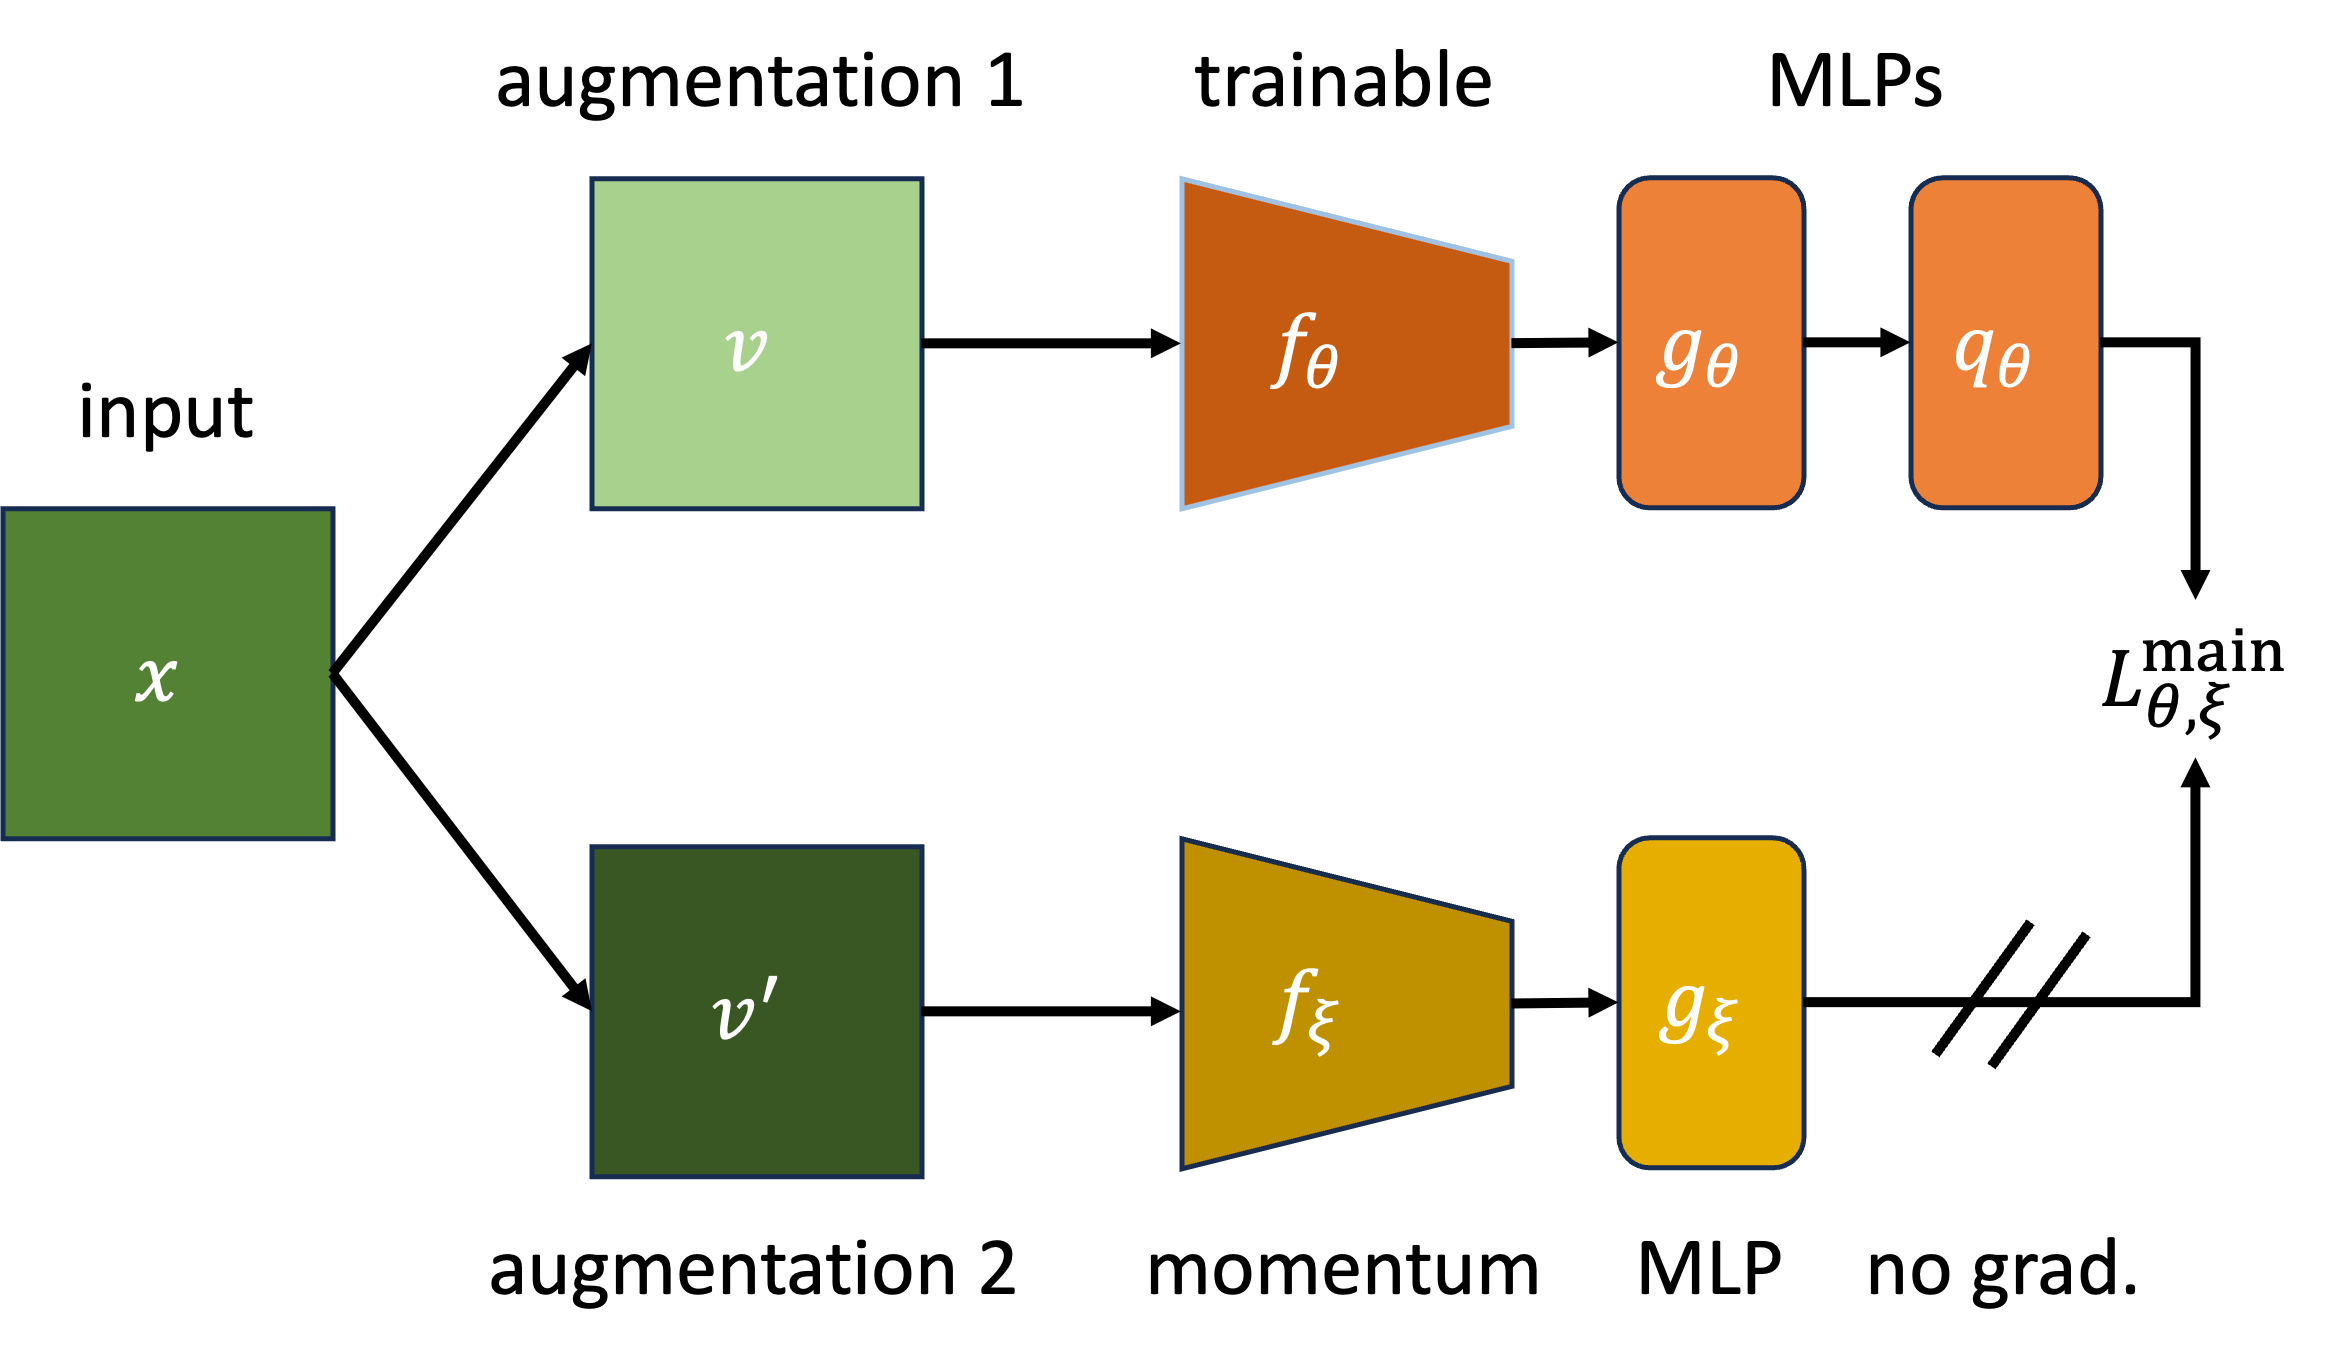
\includegraphics[width=\textwidth]{images/rl1.png}
        \caption{main loss calculation}
        \label{fig:main loss}
    \end{subfigure}
    \hspace{0.02\textwidth} % Adjust space here
    % Second subfigure
    \begin{subfigure}[b]{0.48\textwidth}
        \centering
        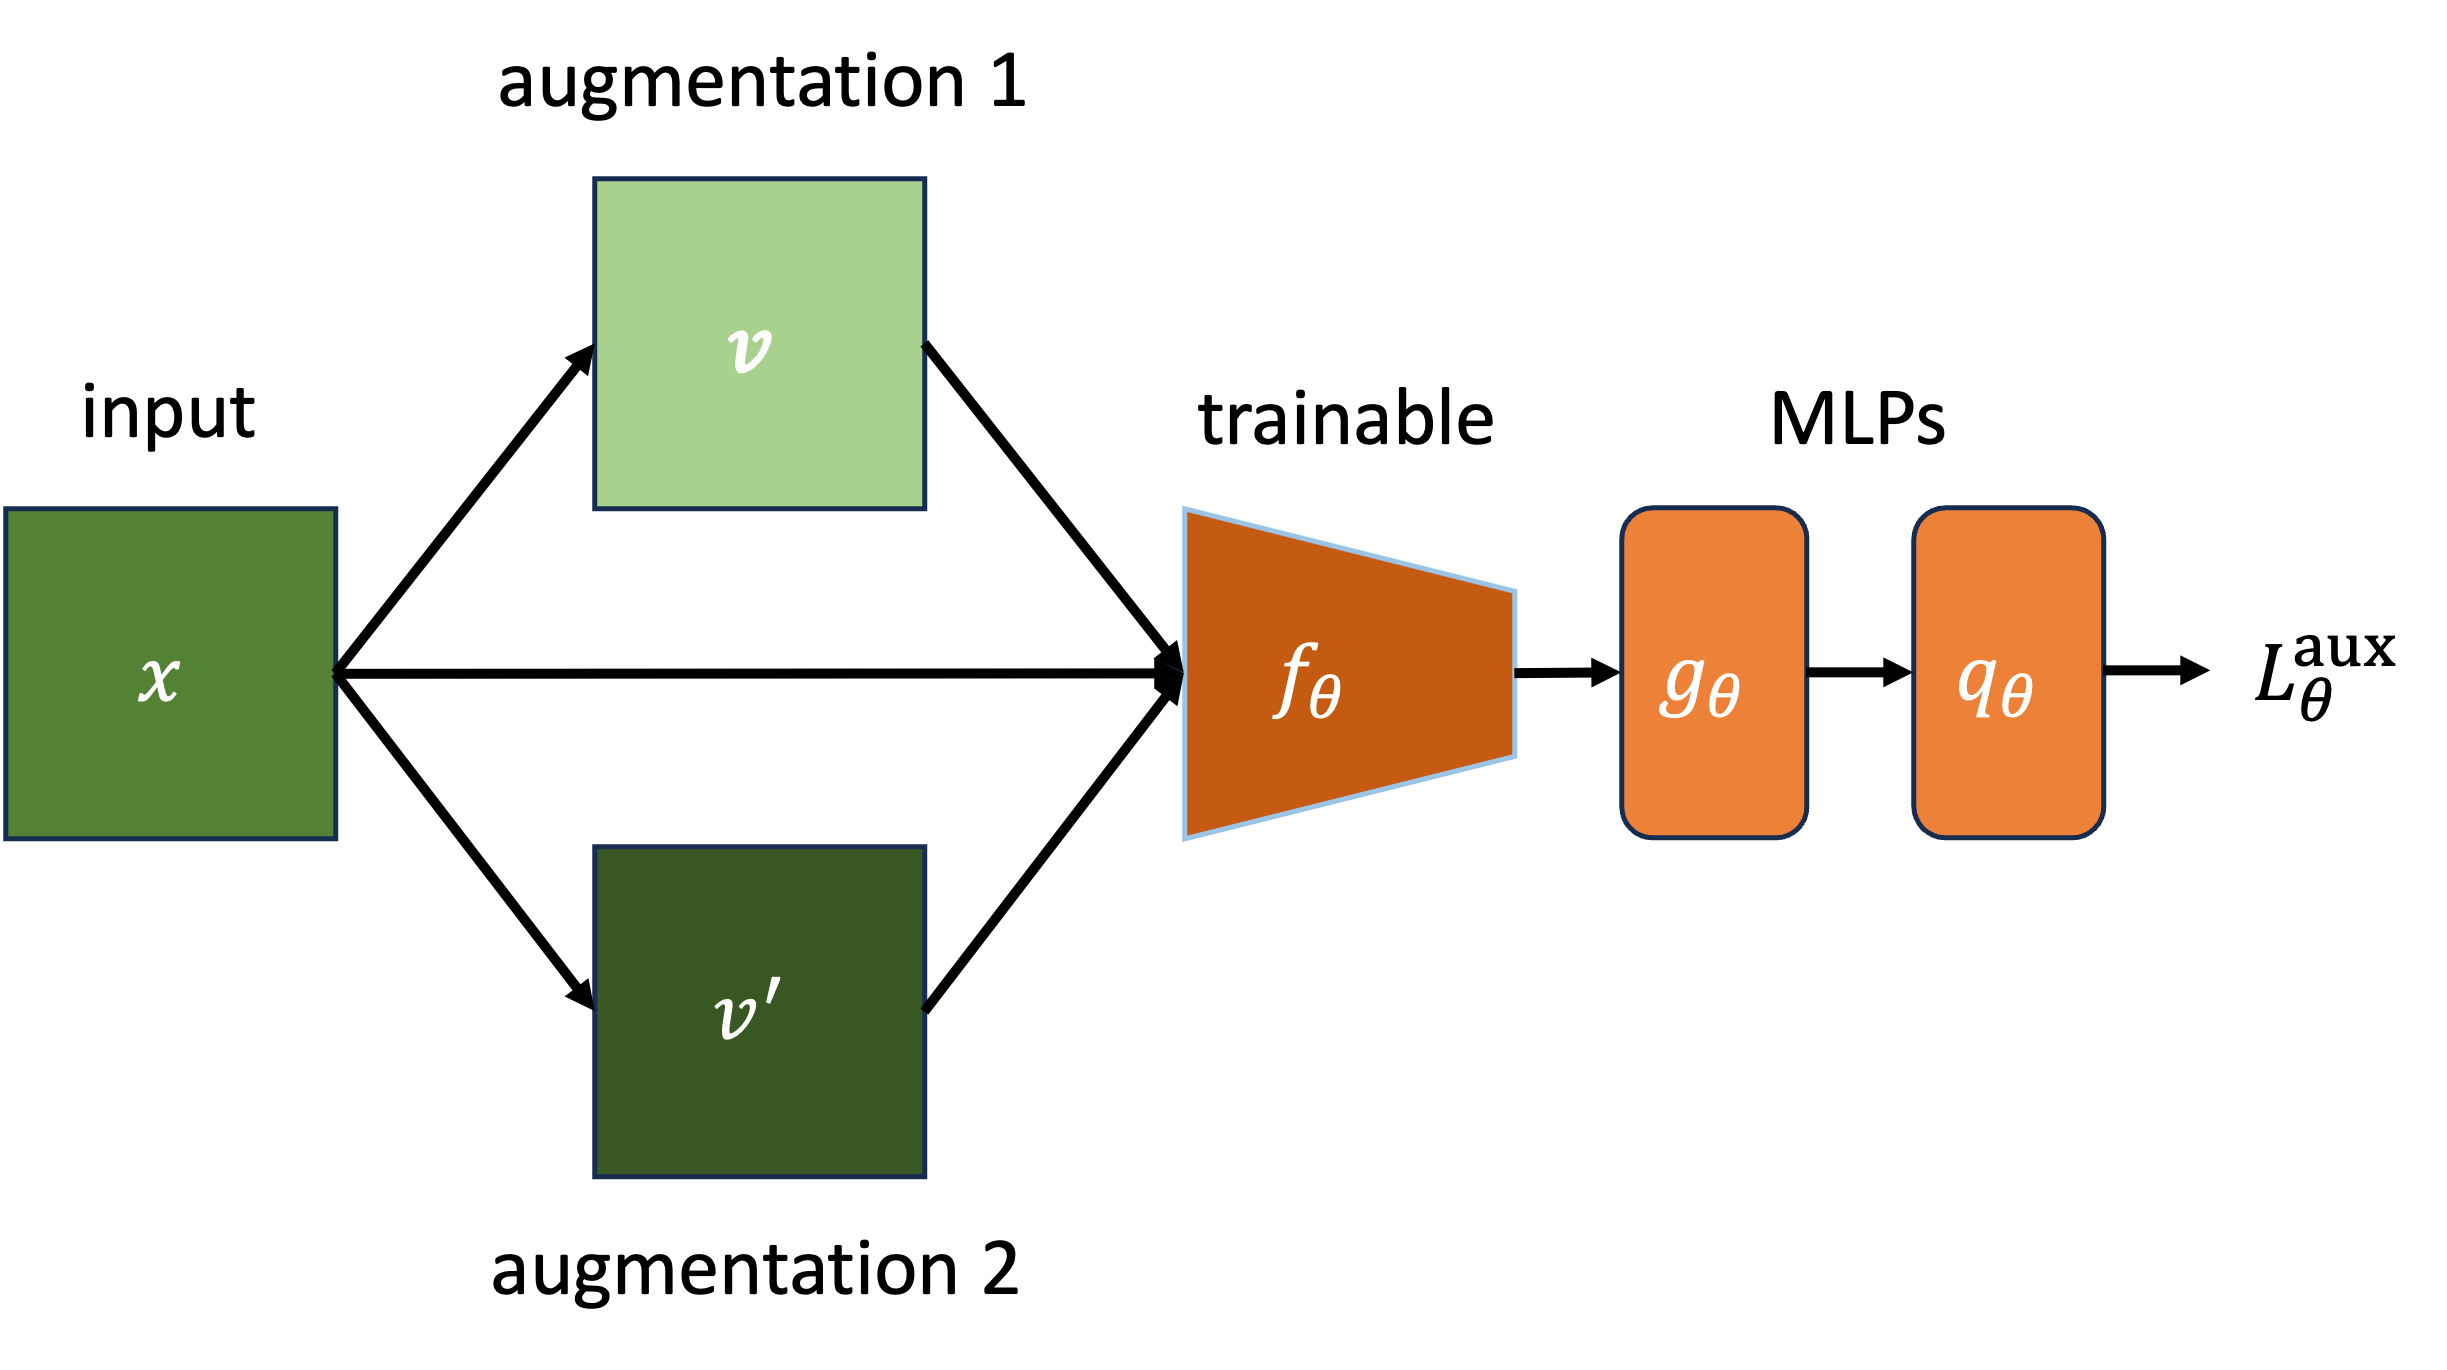
\includegraphics[width=\textwidth]{images/rl2.png}
        \caption{auxiliary loss calculation}
        \label{fig:aux loss}
    \end{subfigure}
    
    \caption{Representation learning with RLPL: \textbf{(a)} The augmented inputs are processed through both networks to compute the main loss. \textbf{(b)} The original and augmented inputs are fed into the trainable network to compute the auxiliary loss.
    }

    \label{fig:two_photos}
\end{figure*}

RLPL learns a representation $y_{\theta}$ for downstream tasks using  encoder $f_{\theta}$, a projector $g_{\theta}$, and a predictor $q_{\theta}$. The momentum network, $f_{\xi}$, with a projector $g_{\xi}$, mirrors the trainable network's architecture but updates as an exponential moving average with decay rate, $\gamma \in [0,1]$:

\begin{equation}
\xi \leftarrow \gamma \xi + (1 - \gamma) \theta.
\end{equation}

For an input image $x$, we create two augmented views $v$ and ${v}'$. The trainable network computes $y_{\theta} \triangleq f_{\theta}(v)$ and $z_{\theta} \triangleq g_{\theta}(y_{\theta})$, while the momentum network outputs $y'_{\xi} \triangleq f_{\xi}(v')$ and $z'_{\xi} \triangleq g_{\xi}(y'_{\xi})$.

We then predict $z'_{\xi}$ from $z_{\theta}$ using $q_{\theta}(z_{\theta})$, and $l_2$-normalize both $q_{\theta}(z_{\theta})$ and $z'_{\xi}$ to $\bar{q}_{\theta}(z_{\theta}) \triangleq \frac{q_{\theta}(z_{\theta})}{\| q_{\theta}(z_{\theta}) \|_{2}}$ and $\bar{z}'_{\xi} \triangleq \frac{z'_{\xi}}{\| z'_{\xi} \|_{2}}$. The loss function is the mean squared error between the normalized prediction and momentum projection (as shown in Figure \ref{fig:main loss}):

\begin{equation} \label{eq:loss}
L_{\theta, \xi} \triangleq \left\| \bar{q}_{\theta}(z_{\theta}) - \bar{z}'_{\xi} \right\|_{2}^{2} = 2 - 2 \cdot \frac{\langle q_{\theta}(z_{\theta}), z'_{\xi} \rangle}{\| q_{\theta}(z_{\theta}) \|_{2} \cdot \| z'_{\xi} \|_{2}}.
\end{equation}

To symmetrize the loss, we feed $v'$ to the trainable network and $v$ to the momentum network, computing $\tilde{L}_{\theta, \xi}$. The combined loss for optimization is:

\begin{equation}
L_{\theta, \xi}^{\text{main}} = L_{\theta, \xi} + \tilde{L}_{\theta, \xi}.
\end{equation}

To calculate the auxiliary loss, the original image goes through the online network as an additional input (as shown in Figure \ref{fig:aux loss}). For original input $x$ and augmented views $v, v'$, we obtain outputs $q_{\theta}(z_{\theta }^{x})\triangleq q_{\theta}(g_{\theta}(f_{\theta}(x)))$, $q_{\theta}(z_{\theta }^{v})\triangleq q_{\theta}(g_{\theta}(f_{\theta}(v)))$, and $q_{\theta}(z_{\theta }^{v'})\triangleq q_{\theta}(g_{\theta}(f_{\theta}(v')))$, respectively. We design an auxiliary loss that allows gradient flow during backpropagation. This auxiliary loss is combined with the main loss, weighted by a factor \(\lambda\). The momentum network stays the same, but the trainable network affects its update parameters.

We calculate the mean of two output embeddings, $\bar{q_{\theta}}(z_{\theta }^{vv'})$, from the prediction head.

\begin{equation}
\bar{q_{\theta}}(z_{\theta }^{vv'}) =  \frac{1}{2}\left ( \bar{q_{\theta}}(z_{\theta}^{v}) + \bar{q_{\theta}}(z_{\theta}^{v'}) \right )
\end{equation}
where $\bar{q_{\theta}}(z_{\theta}^{v})$ and $\bar{q_{\theta}}(z_{\theta}^{v'})$ are the batch-mean of their respective embeddings, $q_{\theta}(z_{\theta}^{v})$ and $q_{\theta}(z_{\theta}^{v'})$.

Now, we denote the auxiliary loss as $L_{\theta}^{\text{aux}}$ and it is expressed as,
\begin{equation}
L_{\theta}^{\text{aux}} = \left \| \bar{q_{\theta}}(z_{\theta}^{x}) - \bar{q_{\theta}}(z_{\theta}^{vv'})\right \|_{2}^{2}
\end{equation}

where $\bar{q_{\theta}}(z_{\theta}^{x})$ is the batch-mean of ${q_{\theta}}(z_{\theta}^{x})$.

% \begin{equation}
% \text{mean}(\bar{q_{\Theta}^{v}}(z_{\Theta}), \bar{q_{\Theta}^{v'}}(z_{\Theta})) = \frac{\bar{q_{\Theta}^{v}}(z_{\Theta}) + \bar{q_{\Theta}^{v'}}(z_{\Theta})}{2}.
% \end{equation}

Next, it is added to the main loss with a weight, $\lambda$, to obtain the total loss.

\begin{equation}
L_{\theta, \xi} = L_{\theta, \xi}^{\text{main}} + \lambda L_{\theta}^{\text{aux}}
\end{equation}

% \noindent where $\lambda$ is the weight for the auxiliary loss.

Optimization updates the trainable network parameters $\theta$ with a learning rate $\eta$, while the momentum network parameters are updated as follows:

\begin{equation}
\theta \leftarrow \text{optimizer}(\theta, \nabla_{\theta} L_{\theta, \xi}, \eta),
\end{equation}

\begin{equation}
\xi \leftarrow \gamma \xi + (1 - \gamma) \theta.
\end{equation}

After training, only the encoder $f_{\theta}$ is returned for the downstream tasks. The pseudo-code for these steps is provided in Algorithm \ref{alg:bywl}.

% \begin{figure}[t]
\begin{algorithm}[!htbp]
\caption{Representation learning with RLPL} \label{alg:bywl}
\begin{algorithmic}
\State \textcolor{pythoncomment}{\# f\_t: trainable net (backbone + projector + predictor)}
\State \textcolor{pythoncomment}{\# f\_m: momentum net (backbone + projector)}
\State \textcolor{pythoncomment}{\# lambda: weight of auxiliary loss}
\State \textcolor{pythoncomment}{\# gma: momentum update rate}

\State \text{}
\State \textcolor{pythoncomment}{\# load a minibatch x with n samples}
\State  \textcolor{pythonfunction}{for} x \textcolor{pythonfunction}{in} loader:
\State \hspace{1.1em} v1, v2 = augment(x) \textcolor{pythoncomment}{\# two random augmentations}

\State \text{}
\State \hspace{1.1em} \textcolor{pythoncomment}{\# compute embeddings}
\State \hspace{1.1em}	t, t1, t2 = f\_t(x), f\_t(v1), f\_t(v2)  , \textcolor{pythoncomment}{\# $N \times D$}

\State \text{}
\State \hspace{1.1em}	\textcolor{purpleish}{with} torch.no\_grad(): \textcolor{pythoncomment}{\# stop the gradient}
\State \hspace{2.5em}	m1, m2 = f\_m(v1), f\_m(v2) \textcolor{pythoncomment} {\# $N \times D$}

\State \text{}
\State \hspace{1.1em} \textcolor{pythoncomment}{\# calculate the losses}
\State \hspace{1.1em}	loss\_main = (loss1(t1, m2) + loss1(t2, m1)).mean()
\State \hspace{1.1em} loss\_aux = loss2(t, t1, t2)
\State \hspace{1.1em}	total\_loss = loss\_main + lambda * loss\_aux

\State \text{}
\State \hspace{1.1em} \textcolor{pythoncomment}{\# optimization step}
\State \hspace{1.1em} total\_loss.backward() 
\State \hspace{1.1em} update(f\_t.params)

\State \text{}
\State \hspace{1.1em} \textcolor{pythoncomment}{\# momentum network update}
\State \hspace{1.1em} f\_m.params = gma*f\_m.params+(1-gma)*f\_t.params

% \Ensure encoder $f_{\theta}$

\State \text{}

\State \textcolor{pythonfunction}{def} loss1(a, b):  \textcolor{pythoncomment}{\# main loss function}
\State \hspace{1.1em} a = normalize(a, dim=-1)
\State \hspace{1.1em} b = normalize(b, dim=-1)
\State \hspace{1.1em} loss = 2 - 2 * (a * b).\textcolor{pythonfunction}{sum}(dim=-1) 
\State \hspace{1.1em} \textcolor{pythonfunction}{return} loss.mean()

%\State \text{}

\State \textcolor{pythonfunction}{def} loss2(a, b, c): \textcolor{pythoncomment}{\# auxiliary loss function}
\State \hspace{1.1em}	avr\_emb = mean(b, c, dim=-1)
\State \hspace{1.1em} loss = (a - avr\_emb) ** 2)
\State \hspace{1.1em} \textcolor{pythonfunction}{return} loss.mean()
\end{algorithmic}
\end{algorithm}
% \end{figure}

\subsection{Effective Pseudo Labeling}  

For effective pseudo-labeling, let, $f_{\theta_T}$ and $f_{\theta_S}$ denote teacher and student networks initialized with parameters $\theta_T, \theta_S \leftarrow \theta$ from the pretrained encoder. Given a batch of labeled samples $(x_l, y_l) \in \mathcal{D}_l$ and unlabeled samples $x_u \in \mathcal{D}_u$, we formulate an iterative pseudo-labeling framework.

For each iteration, we first compute the student's initial loss on labeled data:

\begin{equation}
L_{s1} = \mathbb{E}_{(x_l,y_l)\sim\mathcal{D}_l}[\text{CE}(f_{\theta_S}(x_l), y_l)]
\end{equation}

For unlabeled data $x_u$, the teacher network generates soft pseudo-labels through weak augmentation $\mathcal{A}$:

\begin{equation}
\hat{y}_u = f_{\theta_T}(\mathcal{A}(x_u))
\end{equation}

To ensure quality of pseudo-labels, we filter predictions based on confidence threshold $\tau$:

\begin{equation}
\mathcal{M}_u = \{(x_u, \hat{y}_u) | \max(f_{\theta_T}(\mathcal{A}(x_u))) \geq \tau\}
\end{equation}

The teacher then learns from the filtered pseudo-labeled data:

\begin{equation}
L_u = \mathbb{E}_{(x_u,\hat{y}_u)\sim\mathcal{M}_u}[\text{CE}(f_{\theta_T}(x_u), \hat{y}_u)]
\end{equation}

After updating the student parameters using $L_u$, we measure its new performance:

\begin{equation}
L_{s2} = \mathbb{E}_{(x_l,y_l)\sim\mathcal{D}_l}[\text{CE}(f_{\theta_S}(x_l), y_l)]
\end{equation}

The effectiveness of pseudo-labeling is captured by the performance change:

\begin{equation}
\Delta L_s = L_{s2} - L_{s1}
\end{equation}

We incorporate this feedback through a meta-loss:

\begin{equation}
L_{\text{meta}} = \Delta L_s \cdot L_u
\end{equation}

The final objective for updating the teacher combines supervised learning on labeled data with the meta-loss feedback:

\begin{equation}
L_{\text{total}} = \underbrace{\mathbb{E}_{(x_l,y_l)\sim\mathcal{D}_l}[\text{CE}(f_{\theta_T}(x_l), y_l)]}_{\text{supervised loss}} + \underbrace{L_{\text{meta}}}_{\text{feedback}}
\end{equation}

This formulation creates a feedback loop where the teacher's pseudo-labeling strategy is dynamically adjusted based on the student's learning outcomes. When $\Delta L_s < 0$, indicating improved student performance, the teacher is encouraged to maintain its current strategy. Conversely, when $\Delta L_s > 0$, suggesting degraded performance, the teacher receives a stronger gradient signal to modify its approach.

The optimization proceeds iteratively:

\begin{align}
\theta_S &\leftarrow \theta_S - \eta_S \nabla_{\theta_S} L_u \\
\theta_T &\leftarrow \theta_T - \eta_T \nabla_{\theta_T} L_{\text{total}}
\end{align}

where $\eta_S$ and $\eta_T$ are learning rates for student and teacher networks respectively. After training convergence, only the teacher network is retained for deployment.

The pseudo-code for our pseudo labeling approach is provided in Algorithm~\ref{alg:PL}.

% \begin{figure}[t]
\begin{algorithm}[!htbp]
\caption{Pseudo labeling with RLPL} \label{alg:PL}
\begin{algorithmic}

\State \textcolor{pythoncomment}{\# f\_t: pretrained encoder}
\State \textcolor{pythoncomment}{\# n\_t, n\_s: teacher and student networks}
\State \textcolor{pythoncomment}{\# tau: pseudo labels threshold}

\State \text{}

\State \textcolor{pythoncomment}{\# initialize teacher and student networks}

\State n\_t = f\_t.state\_dict()
\State n\_s = f\_t.state\_dict()

\State \text{}
\State \textcolor{pythoncomment}{\# load a minibatch of labeled and unlabeled samples}
\State  \textcolor{pythonfunction}{for} x, y, x\_u \textcolor{pythonfunction}{in} loader:
\State \hspace{1.1em}	\textcolor{purpleish}{with} torch.no\_grad(): \textcolor{pythoncomment}{\# stop the gradient}
\State \hspace{2.5em} loss\_s1 = cross\_entropy(n\_s(x), y)
\State \hspace{1.1em} y\_u = n\_t(x\_u) 
\State \hspace{1.1em} \textcolor{pythoncomment}{\# filtering unlabled samples based on threshold}
\State \hspace{1.1em} x\_u, y\_u = x\_u $\left[  \text{y\_u} \geq \text{tau}\right]$, y\_u $\left[  \text{y\_u} \geq \text{tau}\right]$
\State \text{}
\State \hspace{1.1em} y\_ut = n\_t(augment(x\_u))  \textcolor{pythoncomment}{\# weak augmentation}
\State \hspace{1.1em} loss\_t = cross\_entropy(y\_ut, y\_u)
\State \hspace{1.1em} loss\_t.backward()
\State \hspace{1.1em} update(n\_s.params) \textcolor{pythoncomment}{\# student network update}

\State \text{}
\State \hspace{1.1em}	\textcolor{purpleish}{with} torch.no\_grad(): \textcolor{pythoncomment}{\# stop the gradient}
\State \hspace{2.5em} loss\_s2 = cross\_entropy(n\_s(x), y)
\State \hspace{1.1em} change = loss\_s2 - loss\_s1
\State \hspace{1.1em} meta\_loss = change * loss\_t \textcolor{pythoncomment}{\# meta-loss computation}

\State \text{} 
\State \hspace{1.1em} loss = cross\_entropy(n\_t(x), y)
\State \hspace{1.1em} total\_loss = loss + meta\_loss \textcolor{pythoncomment}{\# total loss}

\State \hspace{1.1em} total\_loss.backward()
\State \hspace{1.1em} update(n\_t.params) \textcolor{pythoncomment}{\# teacher network update}

\end{algorithmic}
\end{algorithm}
% \end{figure}

\section{Experiments}

\subsection{Datasets}

In our experiments, we applied STL-10 \cite{singh2019justification}, CIFAR-10 \cite{ho2018cifar10} and SVHN \cite{sermanet2012convolutional} datasets for unlabeled RL training. The STL-10 dataset is specially designed for unsupervised feature learning as it contains $13,000$ labeled images across $10$ classes and $100,000$ unlabeled images. While we used the entire training set of CIFAR-10 and SVHN datasets for RL, we only used $250$, $1,000$, and $4,000$ labeled training samples in downstream classifications. Additional experiments were conducted on 6 other image datasets \cite{krizhevsky2009learning, xiao2017fashionmnist, LFWTech, helber2019eurosat, nilsback2008automated, imagenette2019} with different class numbers.

\subsection{Implementation Details} 

\textbf{Image augmentations:} We adopt an augmentation pipeline similar to SimCLR and BYOL, implemented in PyTorch \cite{paszke2019pytorch}. For geometric transformations, we apply ``RandomResizedCrop" with a scaling factor between \([0.2, 1.0]\) and ``RandomHorizontalFlip" to introduce random horizontal flips. Color augmentations include ``ColorJitter", which modifies brightness, contrast, and saturation by a maximum factor of \(0.4\), and hue by \(0.1\), applied with a probability of \(0.3\). We include ``RandomGrayscale" to convert images to grayscale with a probability of \(0.2\). For blurring, ``GaussianBlur" is applied, using a Gaussian kernel with a standard deviation sampled from \([1.0, 2.0]\), with a \(0.2\) probability. Finally, we normalize the input images using predefined mean and standard deviation values. 

Our experiments reveal that image resolution significantly affects accuracy; thus, we resize all images to \(256 \times 256\). In the PL phase, weak augmentations are applied to the noisy teacher model, involving random horizontal and vertical flips, each with a probability of \(0.25\).

\noindent
\textbf{Architecture:} We use ResNet18 \cite{ayyachamy2019medical}, a more computationally feasible network, designed for GPU computations. This ResNet18 architecture remains consistent across all settings, including representation learning, and pseudo labeling. The MLPs, projection, and prediction layers adhere to the parameters established by BYOL. In PL, the teacher and student networks are initialized from the ResNet18, pre-trained via RL.

\noindent
\textbf{Optimization:} The RL framework was optimized using the Adam optimizer \cite{zhang2018improved}, whereas PL employed the Stochastic Gradient Descent (SGD) optimizer \cite{gower2019sgd}, both with a learning rate set to $0.0003$. The auxiliary loss is weighted at \(0.5\). RL underwent training for $50$ epochs with a batch size of $128$, while PL was trained over $150$ epochs with a batch size of $16$.

\begin{figure}[!htbp]
    \centering
    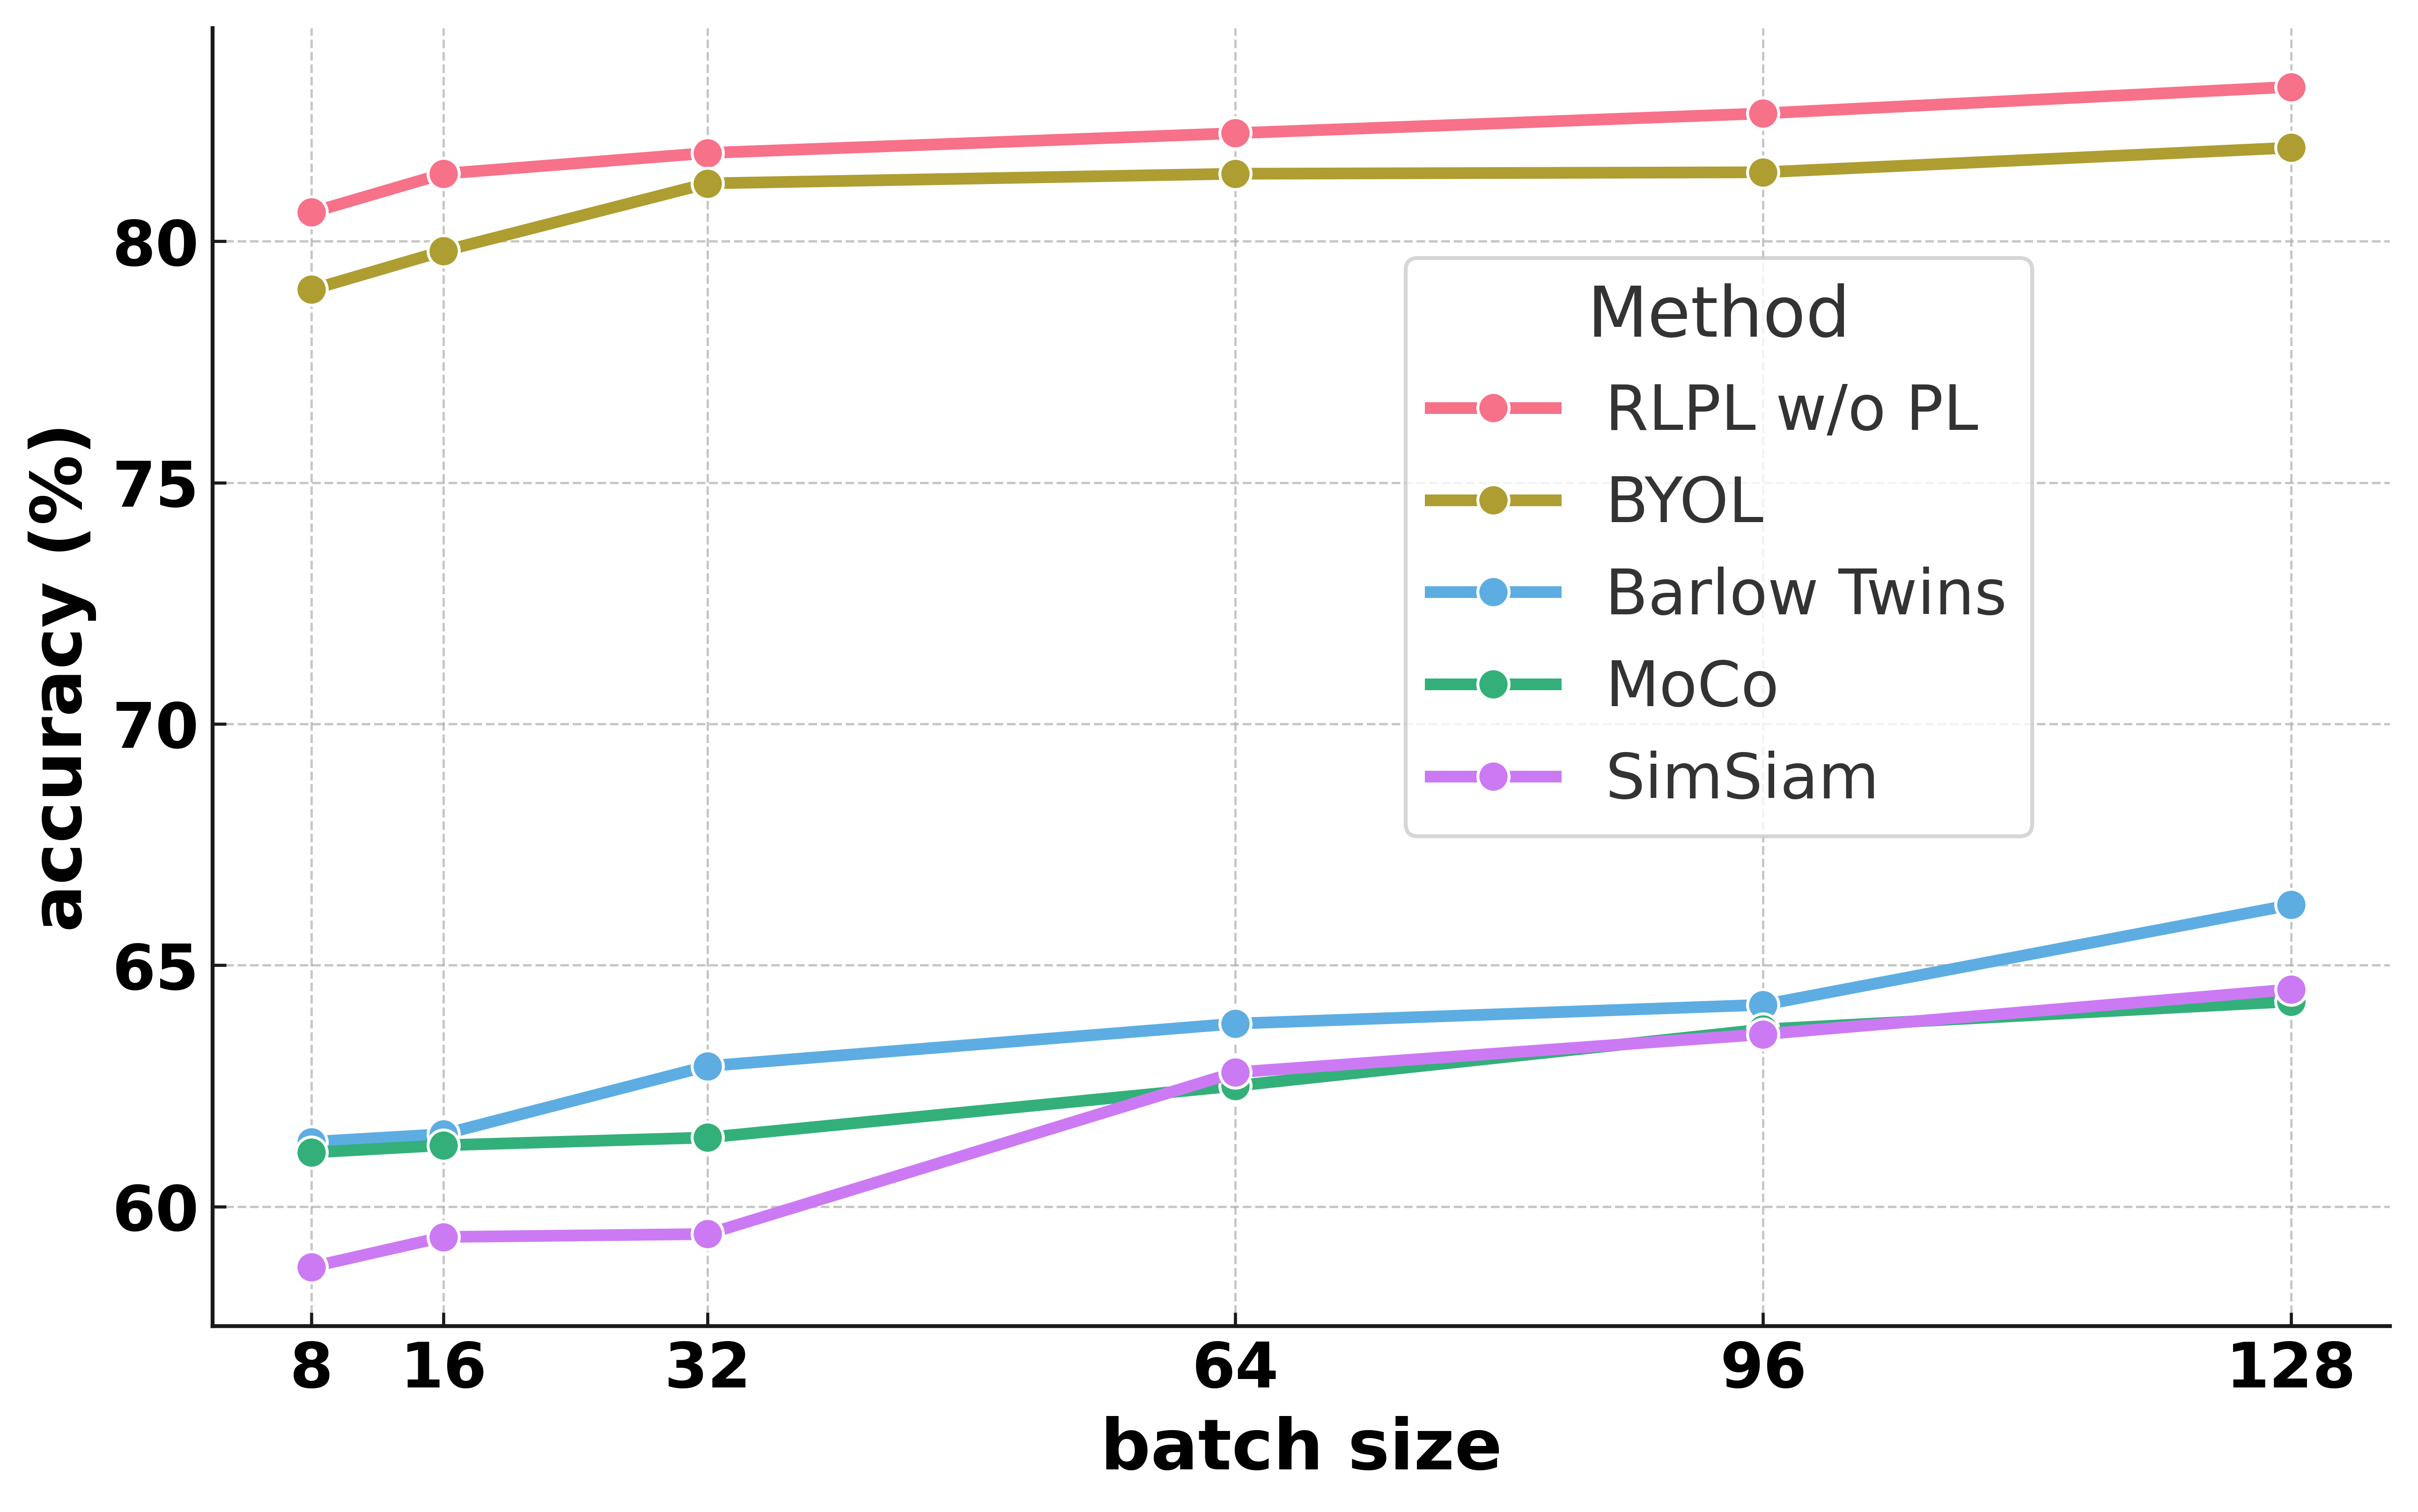
\includegraphics[width=0.9\columnwidth, keepaspectratio]{images/accuracy_vs_batch.png}
    \caption{Effect of batch size on model performance (evaluated on STL-10).}
    \label{fig:batch}
\end{figure}

\begin{table}[htbp]
    \centering
    \begin{tabular}{l c}
      \toprule
      \textbf{Methods} & \textbf{Test Accuracy (\%)} \\  
      \midrule
      Baseline (ResNet18) & 53.16 \\
      FixMatch \cite{sohn2020fixmatch} & 37.28 \\ 
      MixMatch \cite{berthelot2019mixmatch} & 71.60 \\
      MoCo & 66.25 \\
      SimSiam & 64.50 \\
      Barlow Twins & 64.25 \\
      BYOL & 81.94  \\
      RLPL (Ours) & \textbf{84.64} \\
      \bottomrule
    \end{tabular}
    \caption{Performance of different methods on STL-10 dataset.}
    \label{table:stl}
\end{table}

\section{Results and Discussion}

\begin{table*}[htbp]
\centering
\begin{tabular}{llllllll}
\hline
\multirow{2}{*}{\bf Method} & \multicolumn{3}{c}{\bf CIFAR-10}           & \multicolumn{3}{c}{\bf SVHN}          & \multirow{2}{*}{ Average} \\ \cmidrule(lr){2-4}\cmidrule(lr){5-7}
                        & \bf 250 labels & \bf 1000 labels & \bf 4000 labels & \bf 250 labels & \bf 1000 labels & \bf 4000 labels & \\ \hline
ResNet18  & 33.90  & 43.71  & 58.47 & 41.20 & 84.58  & 87.60 & 58.24 \\
MoCO & 34.50 & 46.75  & 61.88 & 30.75  & 83.25 & 89.12 & 57.37 \\
SimSiam & 23.88 & 29.50 & 48.88 & 14.62 & 51.25 & 67.38 & 39.92 \\
Barlow Twins &  35.88 & 47.75  & 63.75 & 21.88 & 79.01 & 88.25 & 56.42 \\
BYOL  & 33.19 & 46.92 & 59.29 & 67.00  & 85.60 & 88.20 & 63.70 \\ 
RLPL (ours)  & \bf  48.93  & \bf 52.45  &  \bf 65.69 & \bf 72.12 & \bf   88.39 & \bf 92.78 & \bf 70.39 \\ \hline
\end{tabular}
\captionof{table}{Test accuracy (\%) of different methods on varying numbers of training samples.}
\label{table:2}
\end{table*}


\begin{table*}[!htbp]
\centering
\resizebox{\textwidth}{!}{
\begin{tabular}{lllllllll}
\hline
\multirow{2}{*}{\bf Method} & \multirow{2}{*}{\bf STL-10} & \multicolumn{3}{c}{\bf CIFAR-10}           & \multicolumn{3}{c}{\bf SVHN} & \multirow{2}{*}{Average} \\ \cmidrule(lr){3-5}\cmidrule(lr){6-8}
                 &       & \bf 250 labels & \bf 1000 labels & \bf 4000 labels & \bf 250 labels & \bf 1000 labels & \bf 4000 labels & \\ \hline
PL (random init.)      &     53.34         &    30.49        &     40.57        &   55.90         &        11.19    &      17.62       &    75.62       &   40.39 \\
RLPL w/o PL      &      83.20        &    34.54       &     48.48        &   59.60          &     71.25      &       85.54      &     89.00      &   67.66 \\
RLPL (ours)    &    \bf 84.64       & \bf  48.93        &   \bf     52.45     &  \bf     65.69      & \bf    72.12       &    \bf   88.39     &  \bf   92.78  & \bf 72.14 \\ \hline
\end{tabular}
}
\captionof{table}{Test accuracy (\%) for ablation on methods.}
\label{table:ablation}
\end{table*}


Our evaluation methods primarily comprise the baseline model, BYOL, SimSiam, MoCo, Barlaw Twins, RLPL, and two additional semi-supervised algorithms, FixMatch \cite{sohn2020fixmatch}, and MixMatch \cite{berthelot2019mixmatch} on the considered datasets. In all our experiments, we re-implemented each algorithm on a ResNet18 backbone with identical hyperparameters to ensure a fair comparison.

\subsection{Effect of Batch Size}

To illustrate the effectiveness of RLPL with reduced batch sizes, we present the results in Figure \ref{fig:batch}. We started with a batch size of $8$ for RLPL. Subsequently, we gradually increased the batch sizes for RLPL and others to evaluate their performances. To have a fair comparison, we applied the classification tasks only on the learned representation of RL, without any use of PL. As anticipated, the accuracy diminished with smaller batch sizes. Remarkably, at a batch size of $64$, RLPL attained an accuracy of $82.24\%$, surpassing BYOL's accuracy of $81.94\%$ with a batch size of $128$. All other methods, including Barlow Twins, MoCo, and SimSiam, achieve significantly lower accuracy in the small-scale implementation, with their performance further declining as batch size decreases. Although all methods exhibited a decline in accuracy with further reductions in batch sizes, RLPL consistently outperformed BYOL and all the others.

\subsection{Classification Accuracy}

Table \ref{table:stl} reports the classification accuracy on the STL-10 dataset. The ResNet18 classifier demonstrates challenges in reaching acceptable accuracy levels. For a fair comparison, all methods, including FixMatch and MixMatch, were implemented with a ResNet18 backbone and an identical batch size.

The results reveal that FixMatch struggles to achieve competitive accuracy, likely due to the limitations of pseudo-labeling techniques, which often require robust initialization and a deep backbone to perform effectively. While MixMatch shows considerable improvement, it still falls short of the performance attained by BYOL and RLPL. MoCo, SimSiam, and Barlow Twins achieve almost similar but lower accuracy. Notably, BYOL achieves an accuracy of $81.94\%$, whereas RLPL surpasses this with an accuracy of $84.64\%$, obtaining a $\textbf{2.7\%}$ improvement over BYOL.

Table \ref{table:2} compares ResNet18, the four primary methods central to this study, and RLPL across varying training samples. For both datasets, all methods showed progressively higher accuracies with increasing sample sizes. We observe that our method uniquely achieves acceptable accuracy on CIFAR-10 with only 250 labels, whereas other methods struggle under the same conditions. For SVHN with 250 labels, only BYOL and RLPL reach satisfactory accuracy, while other methods perform notably worse. Notably, Notably, RLPL consistently achieved the highest accuracy across all datasets and under all varying configurations, outperforming other methods in each case.

We include a column displaying the average test accuracy across all setups to provide a comprehensive view of the relative performance of each method. Only BYOL comes close to RLPL's performance; however, it still lags by a margin of \textbf{6.69\%}. Nevertheless, RLPL consistently outperformed BYOL across all scenarios, particularly with smaller sample sizes, with improvement margins ranging from $\textbf{2.79\%}$ to $\textbf{15.74\%}$.

\subsection{Transfer to Other Classification Tasks}

\begin{table*}[htbp]
  \centering
  \begin{tabular}{lccccccc}
  \hline
  \textbf{Method} & \textbf{CIFAR100} & \textbf{FashionMNIST} & \textbf{LFW} & \textbf{EuroSAT} & \textbf{OxfordFlowers102} & \textbf{Imagenette} & Average \\ \hline
  ResNet18 & 58.09 & 94.55 & 85.03 & 93.62 & 38.48 & 80.66 & 75.07 \\
  MoCo & 62.50 & 90.54 & \bf 93.21 & 95.00 & 35.00 & 79.88 & 76.69 \\
  SimSiam & 33.88 & 92.63 & 80.41 & 79.38 & 26.12 & 76.82 & 64.54 \\
  Barlow Twins & 58.75 & 94.38 & 89.19 & 94.62 & 27.88 & 80.38 & 74.87 \\
  BYOL & 63.61 & 93.62 & 80.73 & \bf 96.28 & 49.64 & 86.13 & 78.67 \\
  RLPL w/o PL & \bf 68.08 & \bf 96.01 & 89.33 & 96.03 & \bf 51.67 & \bf 87.94 & \bf 81.51 \\ \hline
  \end{tabular}
  \caption{Performance comparison (\% test accuracy) of methods on various datasets.}
  \label{table:transfer}
\end{table*}

To assess RLPL's generalization capabilities, we evaluated it on a range of classification tasks across diverse datasets, as summarized in Table \ref{table:transfer}. This table compares RLPL's performance with baseline and other methods after pretraining on the STL-10 dataset, followed by the downstream tasks. For a fair comparison, we applied the pretrained RLPL model directly, without using PLs in the classification tasks. This approach highlights RLPL's standalone performance; notably, integrating PL strategies could likely enhance accuracy beyond the presented results.

RLPL achieves the highest accuracy in nearly all cases, except for MoCo on the Labeled Faces in the Wild (LFW) dataset and BYOL on the EuroSAT dataset. RLPL obtains an average accuracy of 81.51\%, substantially outperforming methods like SimSiam and Barlow Twins. Moreover, RLPL obtains $\textbf{2.84\%}$ more accuracy than the closest best method, BYOL, across all the transfer learning tasks. This improvement highlights RLPL's transferability on unseen classification tasks.

\section{Ablation Study}

\subsection{Framework Ablation}

\begin{figure*}[htbp]
    \centering
    \begin{subfigure}[t]{0.4\textwidth}
      \centering
      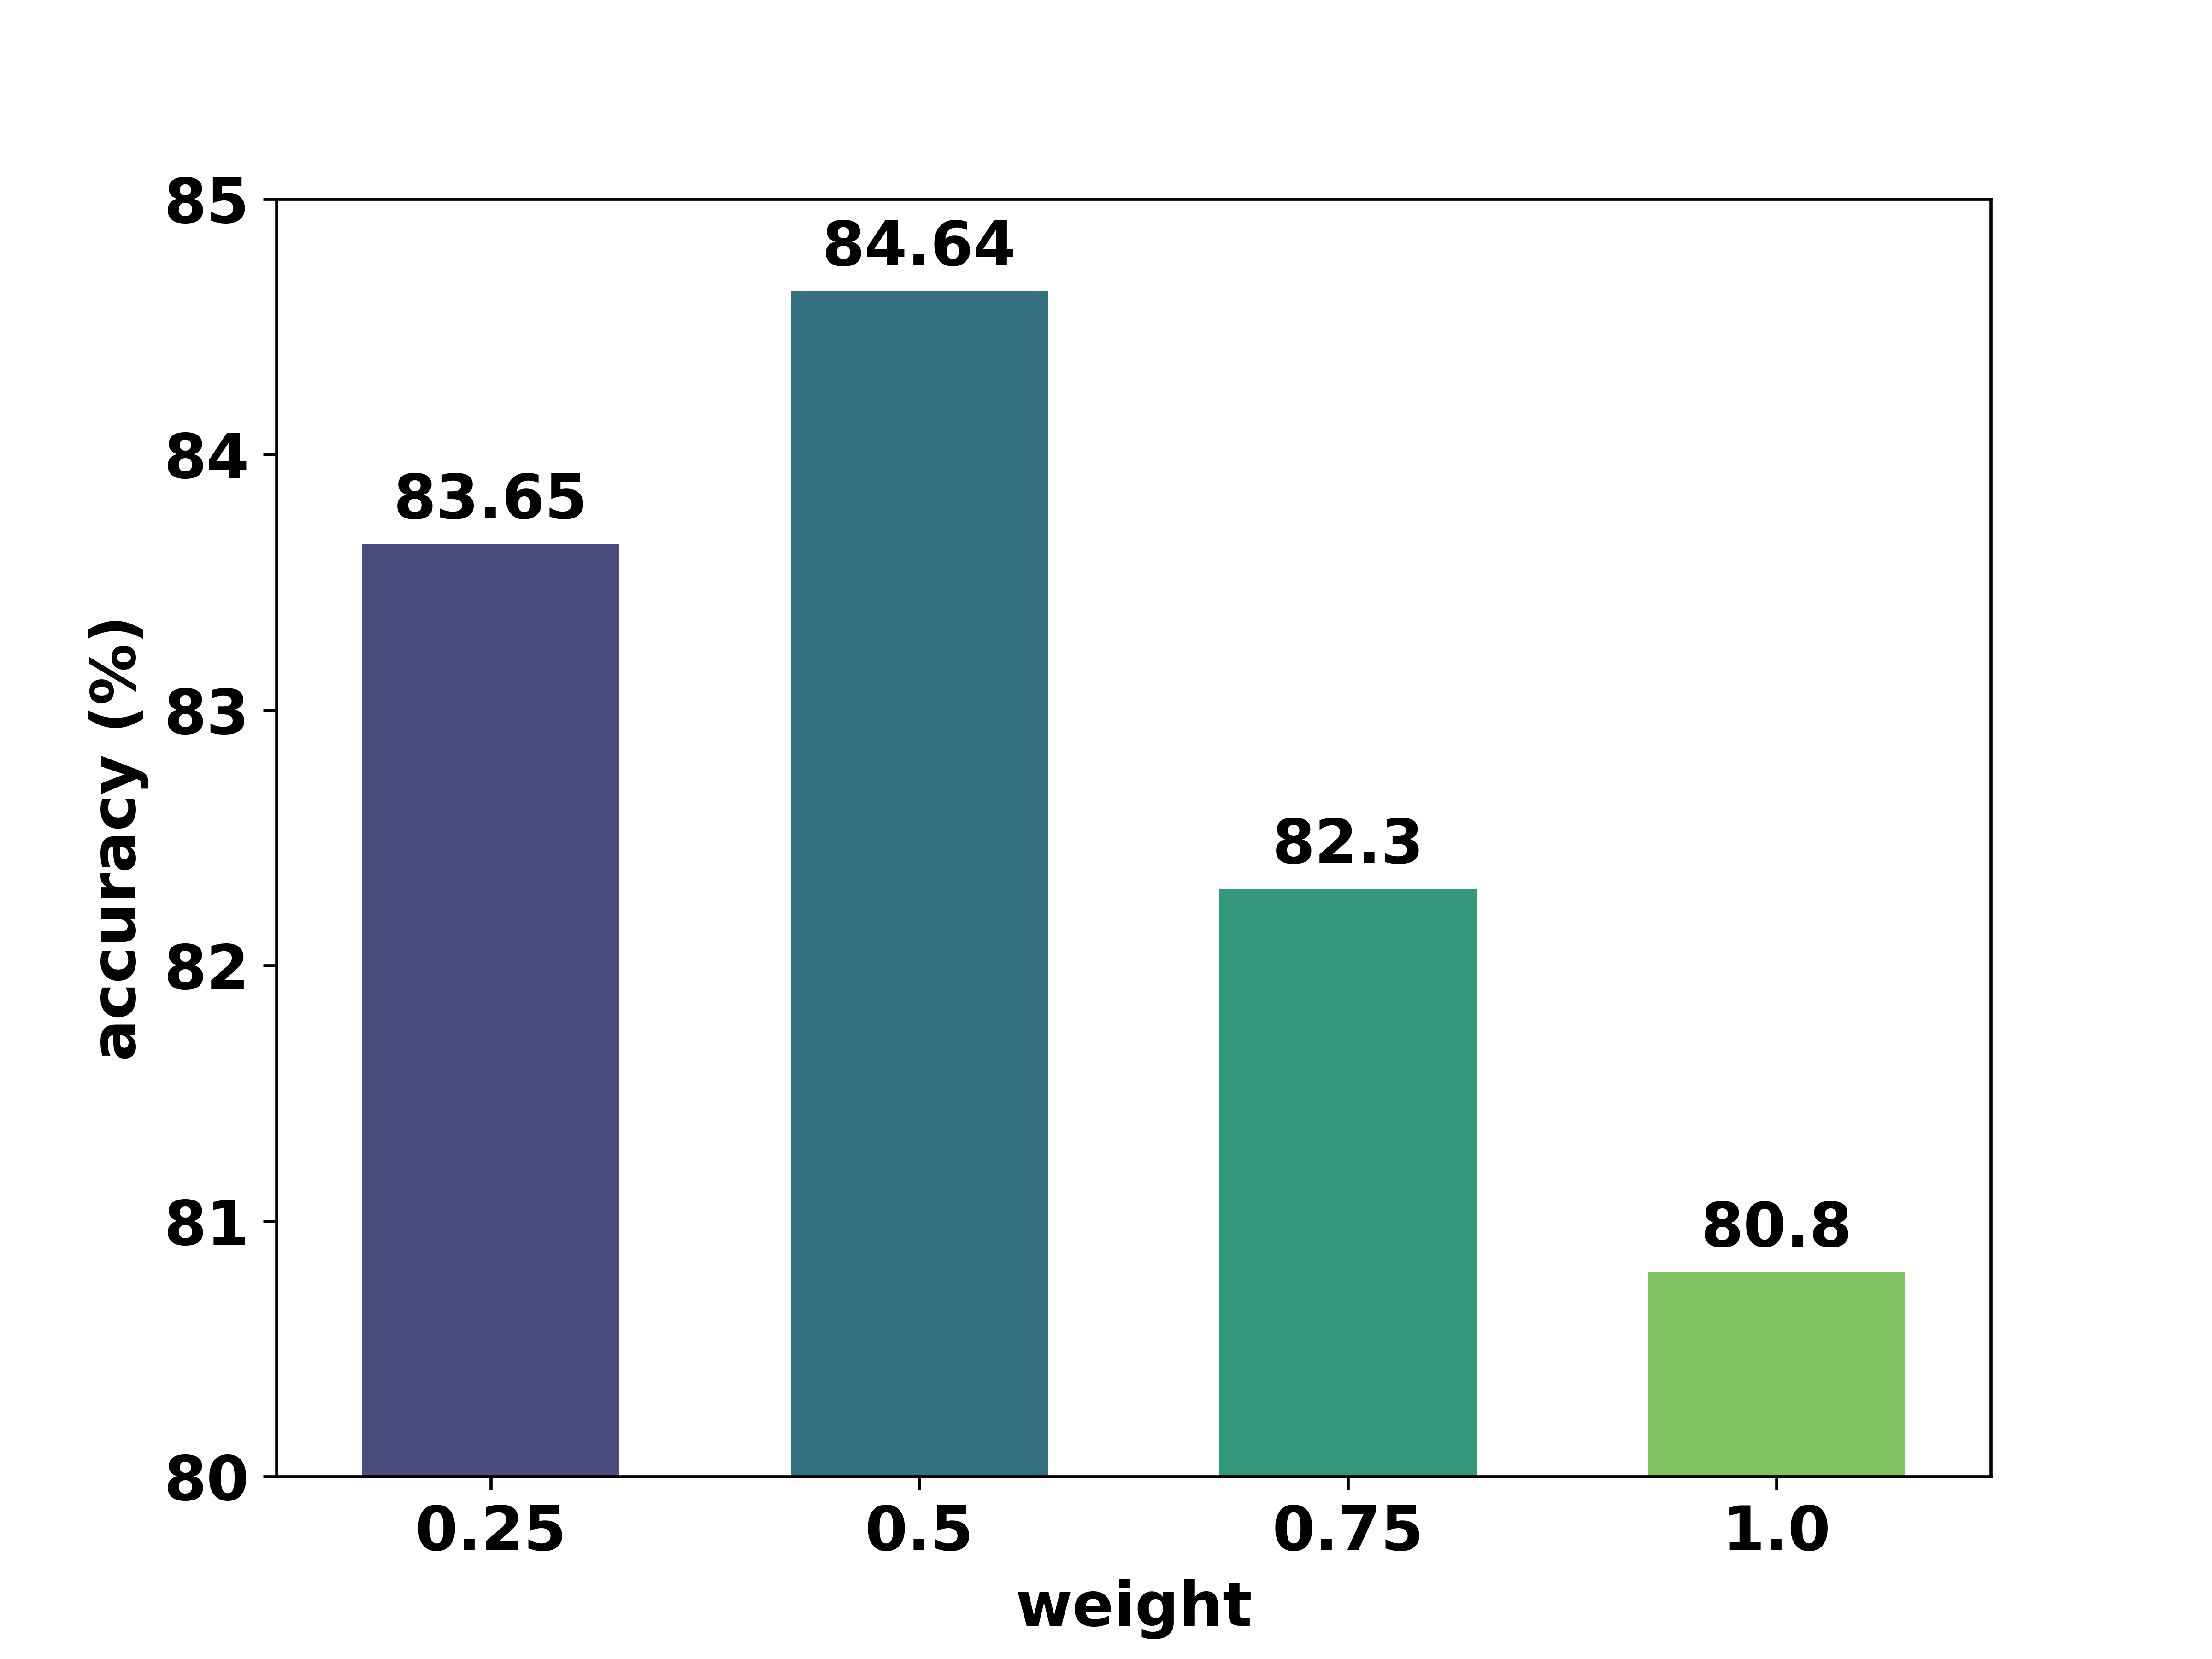
\includegraphics[width=\linewidth]{images/accuracy_vs_weight.png}
      \caption{Effect of the auxiliary loss weight, $\lambda$.}
      \label{fig:weight}
    \end{subfigure}%
  \hspace{0.05\textwidth} % Adjust space here
    \begin{subfigure}[t]{0.4\textwidth}
      \centering
      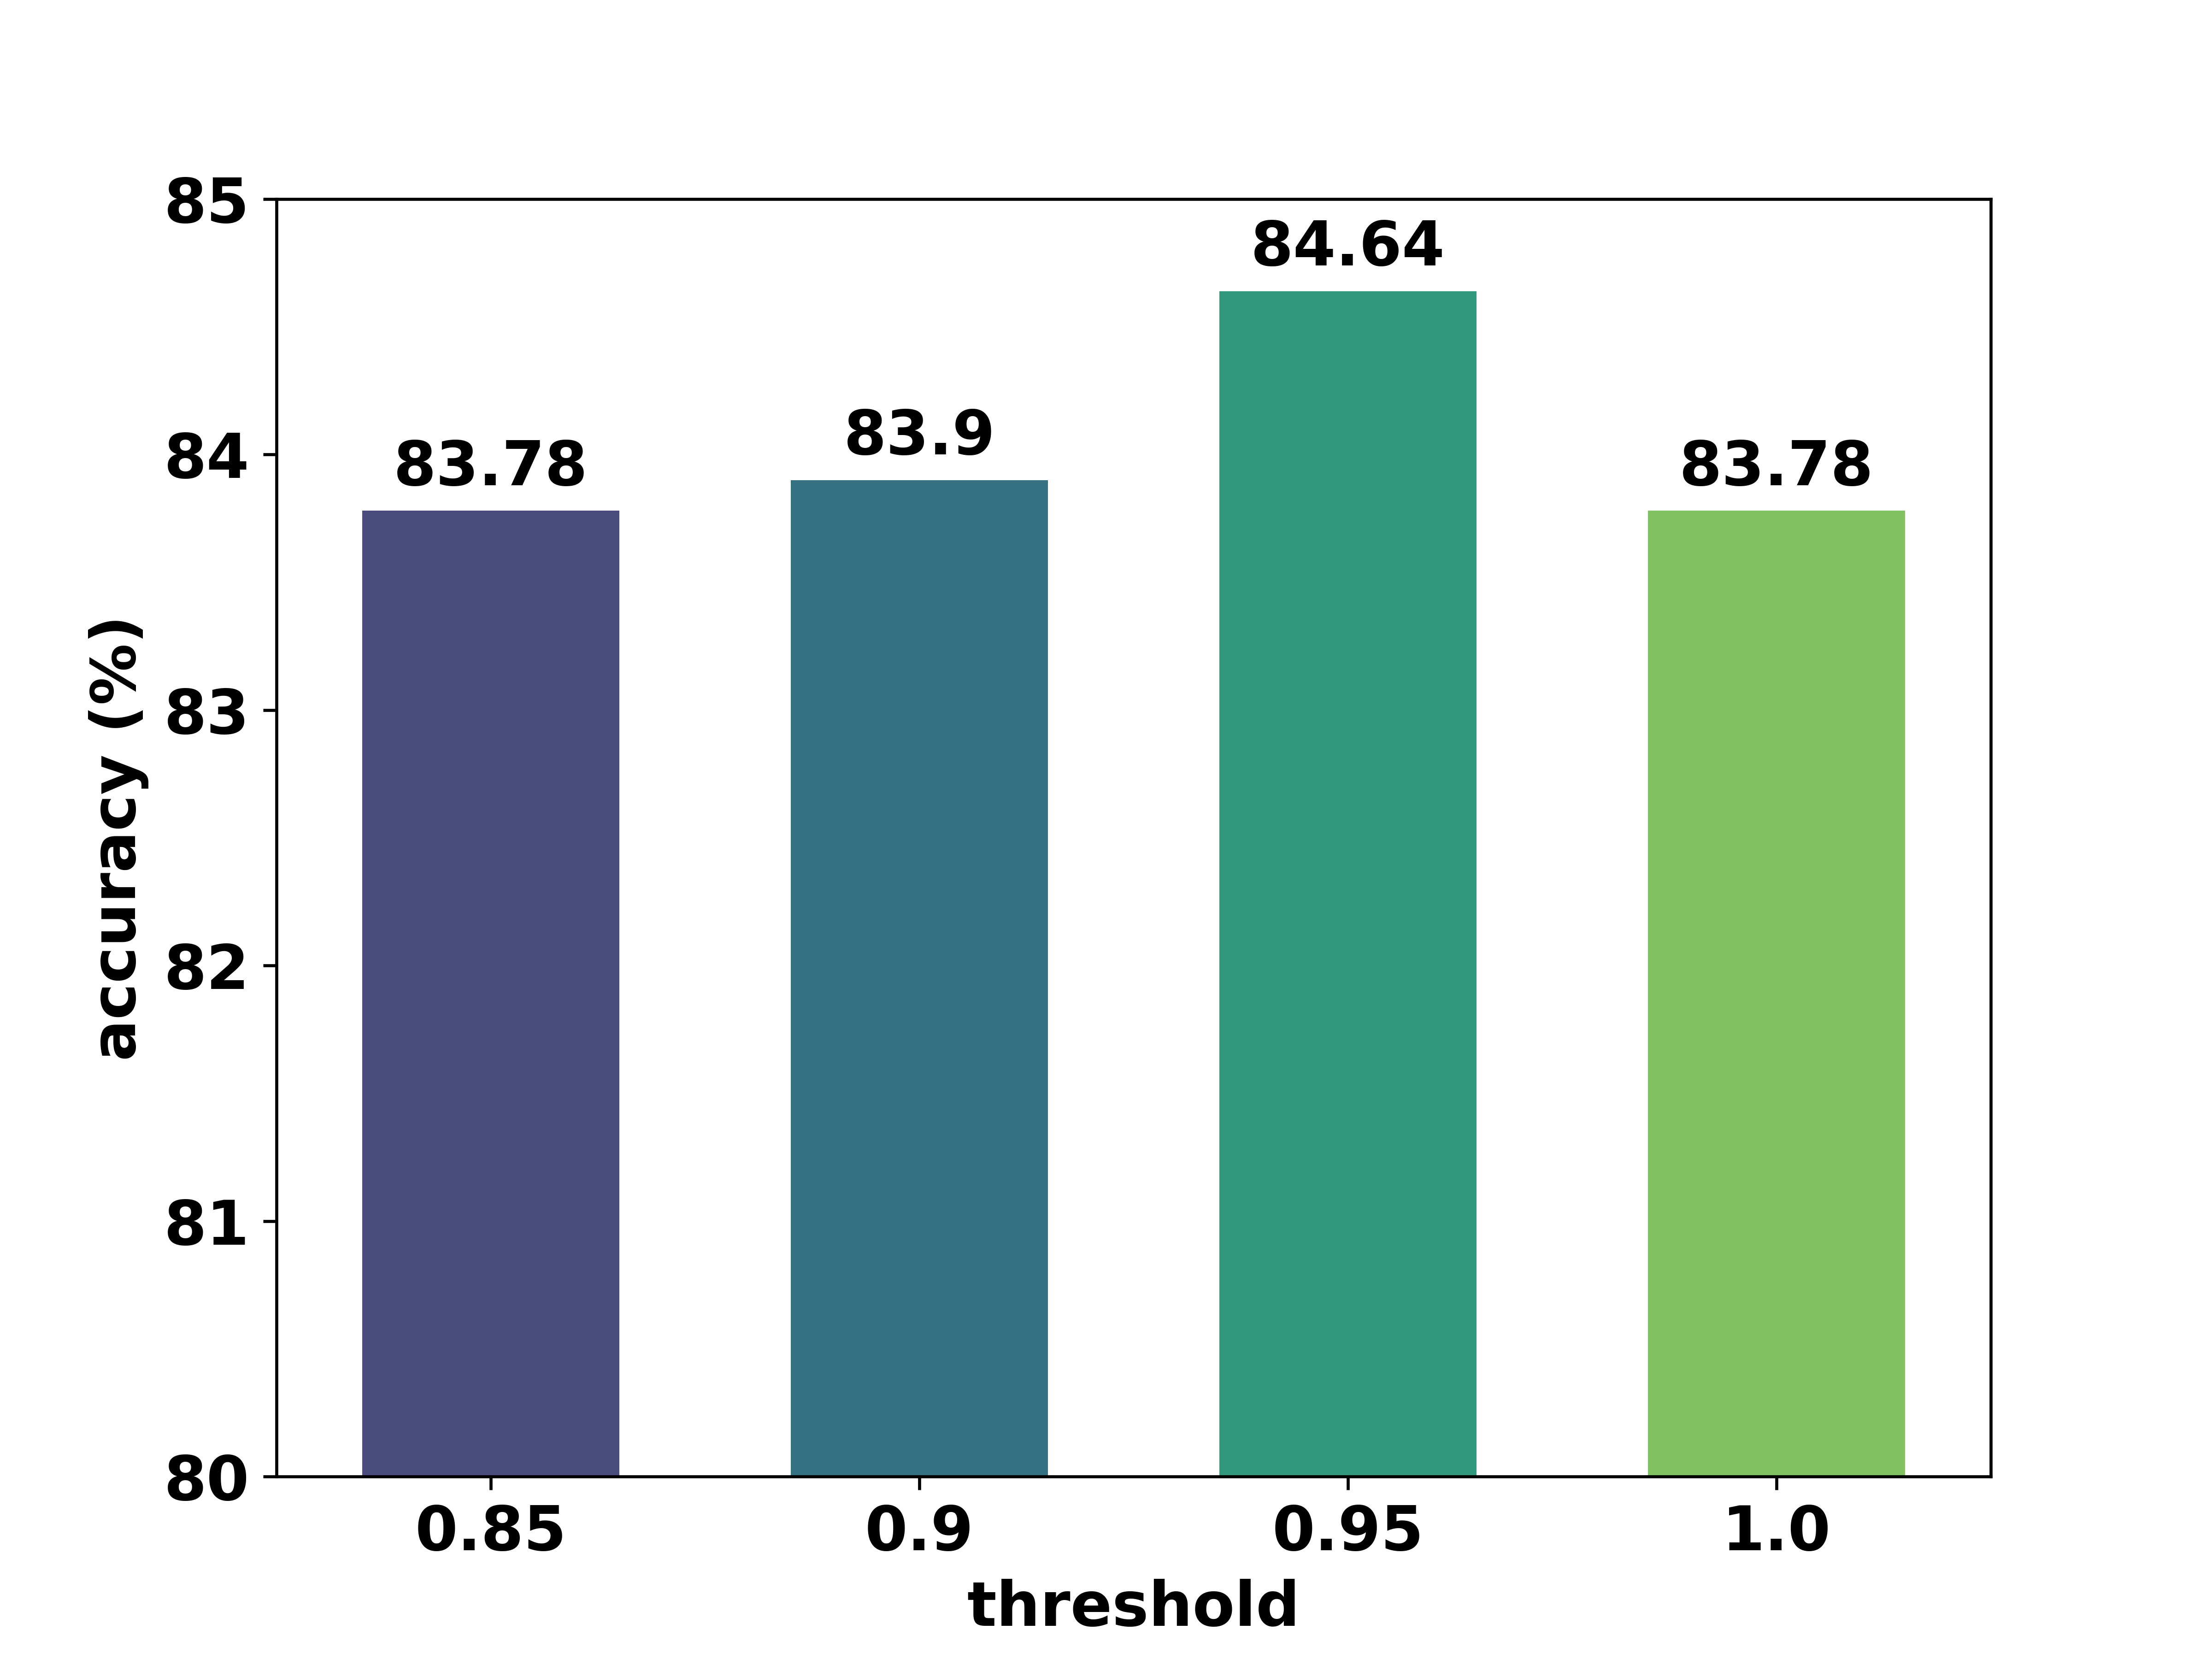
\includegraphics[width=\linewidth]{images/accuracy_vs_threshold.png}
      \caption{Effect of the pseudo labels threshold, $\tau$.}
      \label{fig:threshold}
    \end{subfigure}
    \caption{Effects of different hyperparameters on model performance.}
  \end{figure*}

We conduct extensive ablation studies to evaluate the effectiveness of our method against the PL algorithm with random initialization and RLPL without PLs. Results in Table \ref{table:ablation} demonstrate the consistent superiority of RLPL across diverse datasets and label regimes. The PL with random initialization exhibits limited performance, particularly struggling with low-label scenarios (e.g., 30.49\% and 11.19\% accuracy with 250 labels), highlighting the importance of proper initialization for PL's reliability. 

RLPL without pseudo labeling shows substantial improvements over the baseline, achieving notable gains on STL-10 (83.20\% vs 53.34\%) and SVHN (71.25\% vs 11.19\% for 250 labels), validating the effectiveness of our representation learning strategy. The full RLPL framework, integrating both representation learning and pseudo labeling, consistently achieves the highest performance across all configurations, with particularly strong improvements in low-label settings (e.g., 48.93\% on CIFAR-10 with 250 labels, an 18.44\% improvement). This comprehensive performance advantage is reflected in the average accuracy across all settings, demonstrating RLPL's robust capability, especially in label-scarce scenarios where traditional approaches typically falter.

\subsection{Ablation on Noisy Teacher}

\begin{table}[!htbp]
\centering
\begin{tabular}{cc}
\hline
\textbf{Method} & \textbf{Accuracy (\%)} \\
\hline
Noisy Student    & 84.54 $\pm$ 0.05 \\
Noiseless Teacher & 84.59 $\pm$ 0.02 \\
Noisy Teacher     & 84.63 $\pm$ 0.02 \\
\hline
\end{tabular}
\caption{Input types ablation for pseudo labeling.}
\label{table:noise}
\end{table}

We investigate the impact of noisy samples (weakly augmented) in both teacher and student networks. Table \ref{table:noise} presents the average performance of five different runs for three configurations: the noisy student, the noiseless teacher, and our proposed noisy teacher method. While the differences are subtle, they reveal interesting patterns in model behavior. The noisy student achieves 84.54\% accuracy with a standard deviation of 0.05, suggesting some variability in performance. When we remove noisy samples from the teacher network, we observe a marginal improvement to 84.59\% with reduced variance. Our proposed approach achieves the highest accuracy at 84.63\% with consistently low variance. These results suggest that weak augmentation in the teacher network inputs can provide additional regularization benefits.


% \subsection{Projector Dimensionality}

\section{Parameter Studies}

\subsection{Weight of the Auxiliary Loss}

We modify the weight of auxiliary loss, $\lambda$, from $0.25$ to $1.0$ with an increment of $0.25$. We observe that there is a strong effect of the weight on model performance. For weights other than $0.50$, the test accuracy declines as we move further from this value. The outputs are shown in Figure \ref{fig:weight}.

\subsection{Threshold for Pseudo Labels}

We vary the threshold, $\tau$, from $0.85$ to $1.0$ with an increment of $0.05$. We observe that the highest accuracy is obtained at $0.95$, and it keeps decreasing for a lower threshold value. Again, the accuracy decreases for a threshold value of $1.0$. For any threshold other than $0.95$, the accuracy drops below 84.0\%. The outputs are shown in Figure \ref{fig:threshold}.

\section{Conclusion}

% We introduced the RLPL framework, a novel approach that maximizes the utility of unlabeled data. RLPL addresses key limitations in current methods, such as dependence on large batch sizes and minimal unlabeled data utilization in downstream tasks. Our experiments show that RLPL consistently outperforms other SOTA methods, achieving superior accuracy with reduced batch sizes, making it an efficient choice for memory-constrained environments. RLPL achieved significant improvements across various datasets, demonstrating a notable average performance gain, especially in scenarios with limited labeled data. Beyond accuracy gains, RLPL exhibits strong transferability, demonstrated by its high performance across a range of diverse downstream classification tasks without requiring pseudo labels for adaptation. Overall, RLPL offers a significant improvement in semi-supervised learning, with enhanced data efficiency, robustness, and transferability, making it ideal for diverse memory-efficient applications and strong cross-task generalization.

We present RLPL, a novel semi-supervised learning framework designed to maximize the utility of unlabeled data, addressing critical limitations in existing methods such as the reliance on large batch sizes and underutilization of unlabeled data in downstream tasks. RLPL demonstrates consistent improvements over SOTA methods, achieving high accuracy with smaller batch sizes, which enhances efficiency for memory-constrained environments. Our experiments show that RLPL yields substantial performance gains across multiple datasets, with notable advantages in settings with limited labeled data. In addition to accuracy improvements, RLPL demonstrates exceptional transferability, achieving strong performance across a diverse range of downstream classification tasks without needing pseudo labels for adaptation. By offering enhanced data efficiency, robustness, and generalization, RLPL is ideally suited for a variety of applications that demand memory efficiency and cross-task adaptability, marking a significant advancement in semi-supervised learning.
{
    \small
    \bibliographystyle{ieeenat_fullname}
    \bibliography{main}
}

% WARNING: do not forget to delete the supplementary pages from your submission 
% \input{sec/X_suppl}

\end{document}
